\documentclass[twoside]{book}

% Packages required by doxygen
\usepackage{calc}
\usepackage{doxygen}
\usepackage{graphicx}
\usepackage[utf8]{inputenc}
\usepackage{makeidx}
\usepackage{multicol}
\usepackage{multirow}
\usepackage{textcomp}
\usepackage[table]{xcolor}

% Font selection
\usepackage[T1]{fontenc}
\usepackage{mathptmx}
\usepackage[scaled=.90]{helvet}
\usepackage{courier}
\usepackage{amssymb}
\usepackage{sectsty}
\renewcommand{\familydefault}{\sfdefault}
\allsectionsfont{%
  \fontseries{bc}\selectfont%
  \color{darkgray}%
}
\renewcommand{\DoxyLabelFont}{%
  \fontseries{bc}\selectfont%
  \color{darkgray}%
}

% Page & text layout
\usepackage{geometry}
\geometry{%
  a4paper,%
  top=2.5cm,%
  bottom=2.5cm,%
  left=2.5cm,%
  right=2.5cm%
}
\tolerance=750
\hfuzz=15pt
\hbadness=750
\setlength{\emergencystretch}{15pt}
\setlength{\parindent}{0cm}
\setlength{\parskip}{0.2cm}
\makeatletter
\renewcommand{\paragraph}{%
  \@startsection{paragraph}{4}{0ex}{-1.0ex}{1.0ex}{%
    \normalfont\normalsize\bfseries\SS@parafont%
  }%
}
\renewcommand{\subparagraph}{%
  \@startsection{subparagraph}{5}{0ex}{-1.0ex}{1.0ex}{%
    \normalfont\normalsize\bfseries\SS@subparafont%
  }%
}
\makeatother

% Headers & footers
\usepackage{fancyhdr}
\pagestyle{fancyplain}
\fancyhead[LE]{\fancyplain{}{\bfseries\thepage}}
\fancyhead[CE]{\fancyplain{}{}}
\fancyhead[RE]{\fancyplain{}{\bfseries\leftmark}}
\fancyhead[LO]{\fancyplain{}{\bfseries\rightmark}}
\fancyhead[CO]{\fancyplain{}{}}
\fancyhead[RO]{\fancyplain{}{\bfseries\thepage}}
\fancyfoot[LE]{\fancyplain{}{}}
\fancyfoot[CE]{\fancyplain{}{}}
\fancyfoot[RE]{\fancyplain{}{\bfseries\scriptsize Generated on Sat Jul 6 2013 18:10:00 for ZIM by Doxygen }}
\fancyfoot[LO]{\fancyplain{}{\bfseries\scriptsize Generated on Sat Jul 6 2013 18:10:00 for ZIM by Doxygen }}
\fancyfoot[CO]{\fancyplain{}{}}
\fancyfoot[RO]{\fancyplain{}{}}
\renewcommand{\footrulewidth}{0.4pt}
\renewcommand{\chaptermark}[1]{%
  \markboth{#1}{}%
}
\renewcommand{\sectionmark}[1]{%
  \markright{\thesection\ #1}%
}

% Indices & bibliography
\usepackage{natbib}
\usepackage[titles]{tocloft}
\setcounter{tocdepth}{3}
\setcounter{secnumdepth}{5}
\makeindex

% Hyperlinks (required, but should be loaded last)
\usepackage{ifpdf}
\ifpdf
  \usepackage[pdftex,pagebackref=true]{hyperref}
\else
  \usepackage[ps2pdf,pagebackref=true]{hyperref}
\fi
\hypersetup{%
  colorlinks=true,%
  linkcolor=blue,%
  citecolor=blue,%
  unicode%
}

% Custom commands
\newcommand{\clearemptydoublepage}{%
  \newpage{\pagestyle{empty}\cleardoublepage}%
}


%===== C O N T E N T S =====

\begin{document}

% Titlepage & ToC
\hypersetup{pageanchor=false}
\pagenumbering{roman}
\begin{titlepage}
\vspace*{7cm}
\begin{center}%
{\Large Z\-I\-M }\\
\vspace*{1cm}
{\large Generated by Doxygen 1.8.4}\\
\vspace*{0.5cm}
{\small Sat Jul 6 2013 18:10:00}\\
\end{center}
\end{titlepage}
\clearemptydoublepage
\tableofcontents
\clearemptydoublepage
\pagenumbering{arabic}
\hypersetup{pageanchor=true}

%--- Begin generated contents ---
\chapter{Z\-I\-M}
\label{md_C:_Users_Igor_Android_workspace_ZIM_README}
\hypertarget{md_C:_Users_Igor_Android_workspace_ZIM_README}{}
Z\-I\-M is an android application developed by students of the Otto-\/von-\/\-Guericke-\/\-University Magdeburg for survey purposes concerning \char`\"{}social intelligence\char`\"{}.

\subsection*{Building the project }

In order to build the project on your machine you need to have
\begin{DoxyItemize}
\item google-\/gson
\item Action\-Bar\-Sherlock
\end{DoxyItemize}

\subsection*{Installing the app }

Read the manual for more information about installing and using the app.

\subsection*{Testing }

To run the junit tests you have to create a seperate java project referencing to the \char`\"{}test\char`\"{} folder. This project uses robolectric for unit testing. Check \href{http://pivotal.github.io/robolectric/}{\tt http\-://pivotal.\-github.\-io/robolectric/} for further information 
\chapter{Namespace Index}
\section{Packages}
Here are the packages with brief descriptions (if available)\-:\begin{DoxyCompactList}
\item\contentsline{section}{\hyperlink{namespacecom_1_1ovgu_1_1zim}{com.\-ovgu.\-zim} }{\pageref{namespacecom_1_1ovgu_1_1zim}}{}
\end{DoxyCompactList}

\chapter{Hierarchical Index}
\section{Class Hierarchy}
This inheritance list is sorted roughly, but not completely, alphabetically\-:\begin{DoxyCompactList}
\item \contentsline{section}{com.\-ovgu.\-util.\-Alarm\-Setter}{\pageref{classcom_1_1ovgu_1_1util_1_1_alarm_setter}}{}
\item \contentsline{section}{com.\-ovgu.\-util.\-Alarm\-View\-Model}{\pageref{classcom_1_1ovgu_1_1util_1_1_alarm_view_model}}{}
\item \contentsline{section}{com.\-ovgu.\-util.\-Application\-Values}{\pageref{classcom_1_1ovgu_1_1util_1_1_application_values}}{}
\item \contentsline{section}{com.\-ovgu.\-zim.\-Build\-Config}{\pageref{classcom_1_1ovgu_1_1zim_1_1_build_config}}{}
\item \contentsline{section}{com.\-ovgu.\-util.\-C\-S\-V\-Exporter}{\pageref{classcom_1_1ovgu_1_1util_1_1_c_s_v_exporter}}{}
\item \contentsline{section}{com.\-ovgu.\-util.\-Database\-Entry}{\pageref{classcom_1_1ovgu_1_1util_1_1_database_entry}}{}
\item \contentsline{section}{com.\-ovgu.\-jsondb.\-J\-S\-O\-N\-Connector}{\pageref{classcom_1_1ovgu_1_1jsondb_1_1_j_s_o_n_connector}}{}
\item Json\-Deserializer\begin{DoxyCompactList}
\item \contentsline{section}{com.\-ovgu.\-jsondb.\-D\-B\-Entry\-Deserializer}{\pageref{classcom_1_1ovgu_1_1jsondb_1_1_d_b_entry_deserializer}}{}
\end{DoxyCompactList}
\item Json\-Serializer\begin{DoxyCompactList}
\item \contentsline{section}{com.\-ovgu.\-jsondb.\-D\-B\-Entry\-Serializer}{\pageref{classcom_1_1ovgu_1_1jsondb_1_1_d_b_entry_serializer}}{}
\end{DoxyCompactList}
\item \contentsline{section}{com.\-ovgu.\-zim.\-J\-S\-O\-N\-Test}{\pageref{classcom_1_1ovgu_1_1zim_1_1_j_s_o_n_test}}{}
\item \contentsline{section}{com.\-ovgu.\-zim.\-Main\-Activity\-Test}{\pageref{classcom_1_1ovgu_1_1zim_1_1_main_activity_test}}{}
\item \contentsline{section}{com.\-ovgu.\-zim.\-Preference\-Activity\-Test}{\pageref{classcom_1_1ovgu_1_1zim_1_1_preference_activity_test}}{}
\item \contentsline{section}{com.\-actionbarsherlock.\-R}{\pageref{classcom_1_1actionbarsherlock_1_1_r}}{}
\item \contentsline{section}{com.\-ovgu.\-zim.\-R}{\pageref{classcom_1_1ovgu_1_1zim_1_1_r}}{}
\item Broadcast\-Receiver\begin{DoxyCompactList}
\item \contentsline{section}{com.\-ovgu.\-util.\-Alarm\-Receiver}{\pageref{classcom_1_1ovgu_1_1util_1_1_alarm_receiver}}{}
\item \contentsline{section}{com.\-ovgu.\-util.\-Boot\-Receiver}{\pageref{classcom_1_1ovgu_1_1util_1_1_boot_receiver}}{}
\end{DoxyCompactList}
\item Sherlock\-Activity\begin{DoxyCompactList}
\item \contentsline{section}{com.\-ovgu.\-zim.\-Alarm\-Activity}{\pageref{classcom_1_1ovgu_1_1zim_1_1_alarm_activity}}{}
\item \contentsline{section}{com.\-ovgu.\-zim.\-Main\-Activity}{\pageref{classcom_1_1ovgu_1_1zim_1_1_main_activity}}{}
\end{DoxyCompactList}
\item Sherlock\-Preference\-Activity\begin{DoxyCompactList}
\item \contentsline{section}{com.\-ovgu.\-zim.\-Preference\-Activity}{\pageref{classcom_1_1ovgu_1_1zim_1_1_preference_activity}}{}
\end{DoxyCompactList}
\end{DoxyCompactList}

\chapter{Class Index}
\section{Class List}
Here are the classes, structs, unions and interfaces with brief descriptions\-:\begin{DoxyCompactList}
\item\contentsline{section}{\hyperlink{classcom_1_1ovgu_1_1zim_1_1_alarm_activity}{com.\-ovgu.\-zim.\-Alarm\-Activity} }{\pageref{classcom_1_1ovgu_1_1zim_1_1_alarm_activity}}{}
\item\contentsline{section}{\hyperlink{classcom_1_1ovgu_1_1util_1_1_alarm_receiver}{com.\-ovgu.\-util.\-Alarm\-Receiver} }{\pageref{classcom_1_1ovgu_1_1util_1_1_alarm_receiver}}{}
\item\contentsline{section}{\hyperlink{classcom_1_1ovgu_1_1util_1_1_alarm_setter}{com.\-ovgu.\-util.\-Alarm\-Setter} }{\pageref{classcom_1_1ovgu_1_1util_1_1_alarm_setter}}{}
\item\contentsline{section}{\hyperlink{classcom_1_1ovgu_1_1util_1_1_alarm_view_model}{com.\-ovgu.\-util.\-Alarm\-View\-Model} }{\pageref{classcom_1_1ovgu_1_1util_1_1_alarm_view_model}}{}
\item\contentsline{section}{\hyperlink{classcom_1_1ovgu_1_1util_1_1_application_values}{com.\-ovgu.\-util.\-Application\-Values} }{\pageref{classcom_1_1ovgu_1_1util_1_1_application_values}}{}
\item\contentsline{section}{\hyperlink{classcom_1_1ovgu_1_1util_1_1_boot_receiver}{com.\-ovgu.\-util.\-Boot\-Receiver} }{\pageref{classcom_1_1ovgu_1_1util_1_1_boot_receiver}}{}
\item\contentsline{section}{\hyperlink{classcom_1_1ovgu_1_1zim_1_1_build_config}{com.\-ovgu.\-zim.\-Build\-Config} }{\pageref{classcom_1_1ovgu_1_1zim_1_1_build_config}}{}
\item\contentsline{section}{\hyperlink{classcom_1_1ovgu_1_1util_1_1_c_s_v_exporter}{com.\-ovgu.\-util.\-C\-S\-V\-Exporter} }{\pageref{classcom_1_1ovgu_1_1util_1_1_c_s_v_exporter}}{}
\item\contentsline{section}{\hyperlink{classcom_1_1ovgu_1_1util_1_1_database_entry}{com.\-ovgu.\-util.\-Database\-Entry} }{\pageref{classcom_1_1ovgu_1_1util_1_1_database_entry}}{}
\item\contentsline{section}{\hyperlink{classcom_1_1ovgu_1_1jsondb_1_1_d_b_entry_deserializer}{com.\-ovgu.\-jsondb.\-D\-B\-Entry\-Deserializer} }{\pageref{classcom_1_1ovgu_1_1jsondb_1_1_d_b_entry_deserializer}}{}
\item\contentsline{section}{\hyperlink{classcom_1_1ovgu_1_1jsondb_1_1_d_b_entry_serializer}{com.\-ovgu.\-jsondb.\-D\-B\-Entry\-Serializer} }{\pageref{classcom_1_1ovgu_1_1jsondb_1_1_d_b_entry_serializer}}{}
\item\contentsline{section}{\hyperlink{classcom_1_1ovgu_1_1jsondb_1_1_j_s_o_n_connector}{com.\-ovgu.\-jsondb.\-J\-S\-O\-N\-Connector} }{\pageref{classcom_1_1ovgu_1_1jsondb_1_1_j_s_o_n_connector}}{}
\item\contentsline{section}{\hyperlink{classcom_1_1ovgu_1_1zim_1_1_j_s_o_n_test}{com.\-ovgu.\-zim.\-J\-S\-O\-N\-Test} }{\pageref{classcom_1_1ovgu_1_1zim_1_1_j_s_o_n_test}}{}
\item\contentsline{section}{\hyperlink{classcom_1_1ovgu_1_1zim_1_1_main_activity}{com.\-ovgu.\-zim.\-Main\-Activity} }{\pageref{classcom_1_1ovgu_1_1zim_1_1_main_activity}}{}
\item\contentsline{section}{\hyperlink{classcom_1_1ovgu_1_1zim_1_1_main_activity_test}{com.\-ovgu.\-zim.\-Main\-Activity\-Test} }{\pageref{classcom_1_1ovgu_1_1zim_1_1_main_activity_test}}{}
\item\contentsline{section}{\hyperlink{classcom_1_1ovgu_1_1zim_1_1_preference_activity}{com.\-ovgu.\-zim.\-Preference\-Activity} }{\pageref{classcom_1_1ovgu_1_1zim_1_1_preference_activity}}{}
\item\contentsline{section}{\hyperlink{classcom_1_1ovgu_1_1zim_1_1_preference_activity_test}{com.\-ovgu.\-zim.\-Preference\-Activity\-Test} }{\pageref{classcom_1_1ovgu_1_1zim_1_1_preference_activity_test}}{}
\item\contentsline{section}{\hyperlink{classcom_1_1actionbarsherlock_1_1_r}{com.\-actionbarsherlock.\-R} }{\pageref{classcom_1_1actionbarsherlock_1_1_r}}{}
\item\contentsline{section}{\hyperlink{classcom_1_1ovgu_1_1zim_1_1_r}{com.\-ovgu.\-zim.\-R} }{\pageref{classcom_1_1ovgu_1_1zim_1_1_r}}{}
\end{DoxyCompactList}

\chapter{Namespace Documentation}
\hypertarget{namespacecom_1_1ovgu_1_1zim}{\section{Package com.\-ovgu.\-zim}
\label{namespacecom_1_1ovgu_1_1zim}\index{com.\-ovgu.\-zim@{com.\-ovgu.\-zim}}
}
\subsection*{Classes}
\begin{DoxyCompactItemize}
\item 
class \hyperlink{classcom_1_1ovgu_1_1zim_1_1_build_config}{Build\-Config}
\item 
class \hyperlink{classcom_1_1ovgu_1_1zim_1_1_r}{R}
\item 
class \hyperlink{classcom_1_1ovgu_1_1zim_1_1_alarm_activity}{Alarm\-Activity}
\item 
class \hyperlink{classcom_1_1ovgu_1_1zim_1_1_main_activity}{Main\-Activity}
\item 
class \hyperlink{classcom_1_1ovgu_1_1zim_1_1_preference_activity}{Preference\-Activity}
\item 
class \hyperlink{classcom_1_1ovgu_1_1zim_1_1_j_s_o_n_test}{J\-S\-O\-N\-Test}
\item 
class \hyperlink{classcom_1_1ovgu_1_1zim_1_1_main_activity_test}{Main\-Activity\-Test}
\item 
class \hyperlink{classcom_1_1ovgu_1_1zim_1_1_preference_activity_test}{Preference\-Activity\-Test}
\end{DoxyCompactItemize}


\subsection{Detailed Description}
Automatically generated file. D\-O N\-O\-T M\-O\-D\-I\-F\-Y 
\chapter{Class Documentation}
\hypertarget{classcom_1_1ovgu_1_1zim_1_1_alarm_activity}{\section{com.\-ovgu.\-zim.\-Alarm\-Activity Class Reference}
\label{classcom_1_1ovgu_1_1zim_1_1_alarm_activity}\index{com.\-ovgu.\-zim.\-Alarm\-Activity@{com.\-ovgu.\-zim.\-Alarm\-Activity}}
}
Inheritance diagram for com.\-ovgu.\-zim.\-Alarm\-Activity\-:\begin{figure}[H]
\begin{center}
\leavevmode
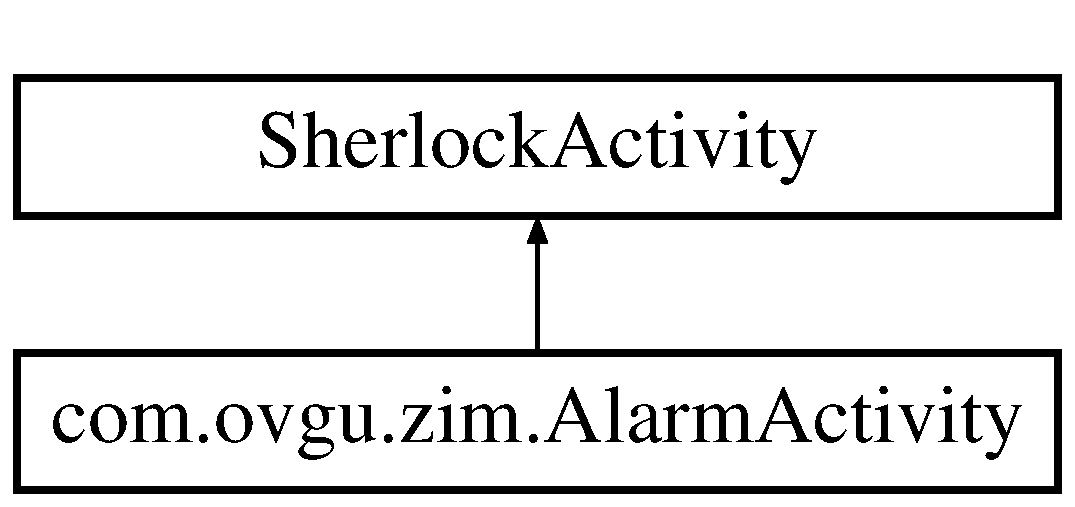
\includegraphics[height=2.000000cm]{classcom_1_1ovgu_1_1zim_1_1_alarm_activity}
\end{center}
\end{figure}
\subsection*{Public Member Functions}
\begin{DoxyCompactItemize}
\item 
boolean \hyperlink{classcom_1_1ovgu_1_1zim_1_1_alarm_activity_a63b6db1ec9db5d4ebc2c73f50d7765cc}{on\-Create\-Options\-Menu} (Menu menu)
\item 
boolean \hyperlink{classcom_1_1ovgu_1_1zim_1_1_alarm_activity_a9636854565b6b5b656b54c129cc25b34}{on\-Options\-Item\-Selected} (Menu\-Item item)
\item 
void \hyperlink{classcom_1_1ovgu_1_1zim_1_1_alarm_activity_a3a5a0f72583d64b2bab175fa7f720e05}{increase\-Contacts1} (View view)
\item 
void \hyperlink{classcom_1_1ovgu_1_1zim_1_1_alarm_activity_ab3fa863a3d90cc3d0ed4944cd3dde0f0}{increase\-Contacts5} (View view)
\item 
void \hyperlink{classcom_1_1ovgu_1_1zim_1_1_alarm_activity_af17eed75579abd860125532d3724d1ff}{increase\-Contacts\-Time5} (View view)
\item 
void \hyperlink{classcom_1_1ovgu_1_1zim_1_1_alarm_activity_ad9a76a33b154f40a5f0086a4ea511b7e}{increase\-Contacts\-Time15} (View view)
\item 
void \hyperlink{classcom_1_1ovgu_1_1zim_1_1_alarm_activity_a235a2bff840877b8fae3d824c7bf437c}{on\-Back\-Pressed} ()
\end{DoxyCompactItemize}
\subsection*{Protected Member Functions}
\begin{DoxyCompactItemize}
\item 
void \hyperlink{classcom_1_1ovgu_1_1zim_1_1_alarm_activity_a922dfea3bce377d5fb7dbc43c975a9c5}{on\-Create} (Bundle saved\-Instance\-State)
\end{DoxyCompactItemize}


\subsection{Detailed Description}
The \hyperlink{classcom_1_1ovgu_1_1zim_1_1_alarm_activity}{Alarm\-Activity} is a Screen\-Activity and is shown after the smartphone user tabs the notification in the notifican bar. The user can enter his amount of contacts and the spend time with them. \begin{DoxyAuthor}{Author}
Igor Lueckel 
\end{DoxyAuthor}


\subsection{Member Function Documentation}
\hypertarget{classcom_1_1ovgu_1_1zim_1_1_alarm_activity_a3a5a0f72583d64b2bab175fa7f720e05}{\index{com\-::ovgu\-::zim\-::\-Alarm\-Activity@{com\-::ovgu\-::zim\-::\-Alarm\-Activity}!increase\-Contacts1@{increase\-Contacts1}}
\index{increase\-Contacts1@{increase\-Contacts1}!com::ovgu::zim::AlarmActivity@{com\-::ovgu\-::zim\-::\-Alarm\-Activity}}
\subsubsection[{increase\-Contacts1}]{\setlength{\rightskip}{0pt plus 5cm}void com.\-ovgu.\-zim.\-Alarm\-Activity.\-increase\-Contacts1 (
\begin{DoxyParamCaption}
\item[{View}]{view}
\end{DoxyParamCaption}
)}}\label{classcom_1_1ovgu_1_1zim_1_1_alarm_activity_a3a5a0f72583d64b2bab175fa7f720e05}
Increases the contact time in the edittext by 1 
\begin{DoxyParams}{Parameters}
{\em view} & \\
\hline
\end{DoxyParams}
\hypertarget{classcom_1_1ovgu_1_1zim_1_1_alarm_activity_ab3fa863a3d90cc3d0ed4944cd3dde0f0}{\index{com\-::ovgu\-::zim\-::\-Alarm\-Activity@{com\-::ovgu\-::zim\-::\-Alarm\-Activity}!increase\-Contacts5@{increase\-Contacts5}}
\index{increase\-Contacts5@{increase\-Contacts5}!com::ovgu::zim::AlarmActivity@{com\-::ovgu\-::zim\-::\-Alarm\-Activity}}
\subsubsection[{increase\-Contacts5}]{\setlength{\rightskip}{0pt plus 5cm}void com.\-ovgu.\-zim.\-Alarm\-Activity.\-increase\-Contacts5 (
\begin{DoxyParamCaption}
\item[{View}]{view}
\end{DoxyParamCaption}
)}}\label{classcom_1_1ovgu_1_1zim_1_1_alarm_activity_ab3fa863a3d90cc3d0ed4944cd3dde0f0}
Increases the contact count in the edittext by 5 
\begin{DoxyParams}{Parameters}
{\em view} & \\
\hline
\end{DoxyParams}
\hypertarget{classcom_1_1ovgu_1_1zim_1_1_alarm_activity_ad9a76a33b154f40a5f0086a4ea511b7e}{\index{com\-::ovgu\-::zim\-::\-Alarm\-Activity@{com\-::ovgu\-::zim\-::\-Alarm\-Activity}!increase\-Contacts\-Time15@{increase\-Contacts\-Time15}}
\index{increase\-Contacts\-Time15@{increase\-Contacts\-Time15}!com::ovgu::zim::AlarmActivity@{com\-::ovgu\-::zim\-::\-Alarm\-Activity}}
\subsubsection[{increase\-Contacts\-Time15}]{\setlength{\rightskip}{0pt plus 5cm}void com.\-ovgu.\-zim.\-Alarm\-Activity.\-increase\-Contacts\-Time15 (
\begin{DoxyParamCaption}
\item[{View}]{view}
\end{DoxyParamCaption}
)}}\label{classcom_1_1ovgu_1_1zim_1_1_alarm_activity_ad9a76a33b154f40a5f0086a4ea511b7e}
Increases the contact time in the edittext by 15 
\begin{DoxyParams}{Parameters}
{\em view} & \\
\hline
\end{DoxyParams}
\hypertarget{classcom_1_1ovgu_1_1zim_1_1_alarm_activity_af17eed75579abd860125532d3724d1ff}{\index{com\-::ovgu\-::zim\-::\-Alarm\-Activity@{com\-::ovgu\-::zim\-::\-Alarm\-Activity}!increase\-Contacts\-Time5@{increase\-Contacts\-Time5}}
\index{increase\-Contacts\-Time5@{increase\-Contacts\-Time5}!com::ovgu::zim::AlarmActivity@{com\-::ovgu\-::zim\-::\-Alarm\-Activity}}
\subsubsection[{increase\-Contacts\-Time5}]{\setlength{\rightskip}{0pt plus 5cm}void com.\-ovgu.\-zim.\-Alarm\-Activity.\-increase\-Contacts\-Time5 (
\begin{DoxyParamCaption}
\item[{View}]{view}
\end{DoxyParamCaption}
)}}\label{classcom_1_1ovgu_1_1zim_1_1_alarm_activity_af17eed75579abd860125532d3724d1ff}
Increases the contact time in the edittext by 5 
\begin{DoxyParams}{Parameters}
{\em view} & \\
\hline
\end{DoxyParams}
\hypertarget{classcom_1_1ovgu_1_1zim_1_1_alarm_activity_a235a2bff840877b8fae3d824c7bf437c}{\index{com\-::ovgu\-::zim\-::\-Alarm\-Activity@{com\-::ovgu\-::zim\-::\-Alarm\-Activity}!on\-Back\-Pressed@{on\-Back\-Pressed}}
\index{on\-Back\-Pressed@{on\-Back\-Pressed}!com::ovgu::zim::AlarmActivity@{com\-::ovgu\-::zim\-::\-Alarm\-Activity}}
\subsubsection[{on\-Back\-Pressed}]{\setlength{\rightskip}{0pt plus 5cm}void com.\-ovgu.\-zim.\-Alarm\-Activity.\-on\-Back\-Pressed (
\begin{DoxyParamCaption}
{}
\end{DoxyParamCaption}
)}}\label{classcom_1_1ovgu_1_1zim_1_1_alarm_activity_a235a2bff840877b8fae3d824c7bf437c}
\hypertarget{classcom_1_1ovgu_1_1zim_1_1_alarm_activity_a922dfea3bce377d5fb7dbc43c975a9c5}{\index{com\-::ovgu\-::zim\-::\-Alarm\-Activity@{com\-::ovgu\-::zim\-::\-Alarm\-Activity}!on\-Create@{on\-Create}}
\index{on\-Create@{on\-Create}!com::ovgu::zim::AlarmActivity@{com\-::ovgu\-::zim\-::\-Alarm\-Activity}}
\subsubsection[{on\-Create}]{\setlength{\rightskip}{0pt plus 5cm}void com.\-ovgu.\-zim.\-Alarm\-Activity.\-on\-Create (
\begin{DoxyParamCaption}
\item[{Bundle}]{saved\-Instance\-State}
\end{DoxyParamCaption}
)\hspace{0.3cm}{\ttfamily [protected]}}}\label{classcom_1_1ovgu_1_1zim_1_1_alarm_activity_a922dfea3bce377d5fb7dbc43c975a9c5}
\hypertarget{classcom_1_1ovgu_1_1zim_1_1_alarm_activity_a63b6db1ec9db5d4ebc2c73f50d7765cc}{\index{com\-::ovgu\-::zim\-::\-Alarm\-Activity@{com\-::ovgu\-::zim\-::\-Alarm\-Activity}!on\-Create\-Options\-Menu@{on\-Create\-Options\-Menu}}
\index{on\-Create\-Options\-Menu@{on\-Create\-Options\-Menu}!com::ovgu::zim::AlarmActivity@{com\-::ovgu\-::zim\-::\-Alarm\-Activity}}
\subsubsection[{on\-Create\-Options\-Menu}]{\setlength{\rightskip}{0pt plus 5cm}boolean com.\-ovgu.\-zim.\-Alarm\-Activity.\-on\-Create\-Options\-Menu (
\begin{DoxyParamCaption}
\item[{Menu}]{menu}
\end{DoxyParamCaption}
)}}\label{classcom_1_1ovgu_1_1zim_1_1_alarm_activity_a63b6db1ec9db5d4ebc2c73f50d7765cc}
\hypertarget{classcom_1_1ovgu_1_1zim_1_1_alarm_activity_a9636854565b6b5b656b54c129cc25b34}{\index{com\-::ovgu\-::zim\-::\-Alarm\-Activity@{com\-::ovgu\-::zim\-::\-Alarm\-Activity}!on\-Options\-Item\-Selected@{on\-Options\-Item\-Selected}}
\index{on\-Options\-Item\-Selected@{on\-Options\-Item\-Selected}!com::ovgu::zim::AlarmActivity@{com\-::ovgu\-::zim\-::\-Alarm\-Activity}}
\subsubsection[{on\-Options\-Item\-Selected}]{\setlength{\rightskip}{0pt plus 5cm}boolean com.\-ovgu.\-zim.\-Alarm\-Activity.\-on\-Options\-Item\-Selected (
\begin{DoxyParamCaption}
\item[{Menu\-Item}]{item}
\end{DoxyParamCaption}
)}}\label{classcom_1_1ovgu_1_1zim_1_1_alarm_activity_a9636854565b6b5b656b54c129cc25b34}


The documentation for this class was generated from the following file\-:\begin{DoxyCompactItemize}
\item 
C\-:/\-Users/\-Igor/\-Android/workspace/\-Z\-I\-M/src/com/ovgu/zim/Alarm\-Activity.\-java\end{DoxyCompactItemize}

\hypertarget{classcom_1_1ovgu_1_1util_1_1_alarm_receiver}{\section{com.\-ovgu.\-util.\-Alarm\-Receiver Class Reference}
\label{classcom_1_1ovgu_1_1util_1_1_alarm_receiver}\index{com.\-ovgu.\-util.\-Alarm\-Receiver@{com.\-ovgu.\-util.\-Alarm\-Receiver}}
}
Inheritance diagram for com.\-ovgu.\-util.\-Alarm\-Receiver\-:\begin{figure}[H]
\begin{center}
\leavevmode
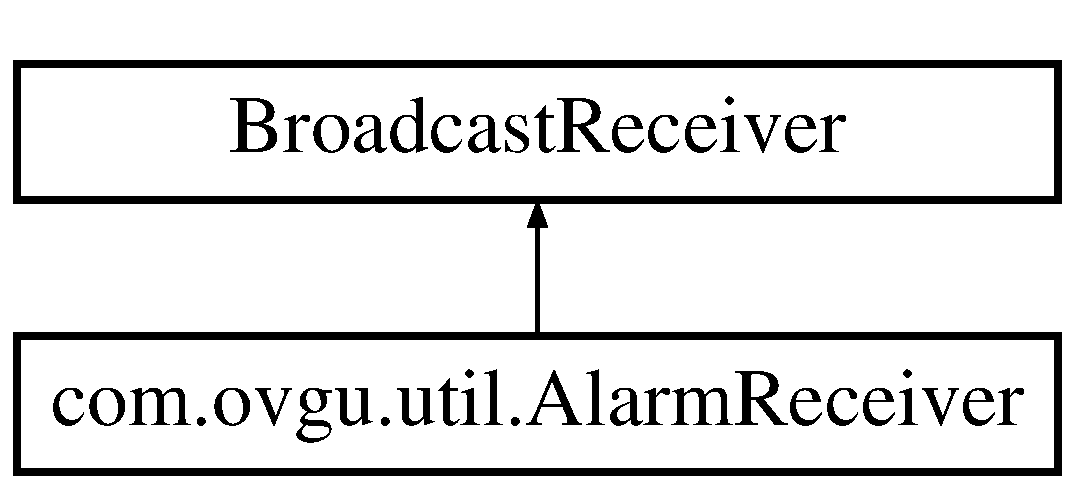
\includegraphics[height=2.000000cm]{classcom_1_1ovgu_1_1util_1_1_alarm_receiver}
\end{center}
\end{figure}
\subsection*{Public Member Functions}
\begin{DoxyCompactItemize}
\item 
void \hyperlink{classcom_1_1ovgu_1_1util_1_1_alarm_receiver_a83312c2f4729f036334c8f84c5af570f}{on\-Receive} (Context context, Intent intent)
\end{DoxyCompactItemize}


\subsection{Detailed Description}
This class gets called if an alarm occures. It plays a sound or vibrates (depends on user preferences) and creates a new notification. \begin{DoxyAuthor}{Author}
Igor Lueckel 
\end{DoxyAuthor}


\subsection{Member Function Documentation}
\hypertarget{classcom_1_1ovgu_1_1util_1_1_alarm_receiver_a83312c2f4729f036334c8f84c5af570f}{\index{com\-::ovgu\-::util\-::\-Alarm\-Receiver@{com\-::ovgu\-::util\-::\-Alarm\-Receiver}!on\-Receive@{on\-Receive}}
\index{on\-Receive@{on\-Receive}!com::ovgu::util::AlarmReceiver@{com\-::ovgu\-::util\-::\-Alarm\-Receiver}}
\subsubsection[{on\-Receive}]{\setlength{\rightskip}{0pt plus 5cm}void com.\-ovgu.\-util.\-Alarm\-Receiver.\-on\-Receive (
\begin{DoxyParamCaption}
\item[{Context}]{context, }
\item[{Intent}]{intent}
\end{DoxyParamCaption}
)}}\label{classcom_1_1ovgu_1_1util_1_1_alarm_receiver_a83312c2f4729f036334c8f84c5af570f}


The documentation for this class was generated from the following file\-:\begin{DoxyCompactItemize}
\item 
C\-:/\-Users/\-Igor/\-Android/workspace/\-Z\-I\-M/src/com/ovgu/util/Alarm\-Receiver.\-java\end{DoxyCompactItemize}

\hypertarget{classcom_1_1ovgu_1_1util_1_1_alarm_setter}{\section{com.\-ovgu.\-util.\-Alarm\-Setter Class Reference}
\label{classcom_1_1ovgu_1_1util_1_1_alarm_setter}\index{com.\-ovgu.\-util.\-Alarm\-Setter@{com.\-ovgu.\-util.\-Alarm\-Setter}}
}
\subsection*{Public Member Functions}
\begin{DoxyCompactItemize}
\item 
void \hyperlink{classcom_1_1ovgu_1_1util_1_1_alarm_setter_a3d9f6595eb50d589ae8cbd6b166cd35f}{set\-Alarms} (Context View)
\item 
void \hyperlink{classcom_1_1ovgu_1_1util_1_1_alarm_setter_aea60dad39f961c9a7b2c89fa0942fd73}{delete\-Alarms} (Context View)
\end{DoxyCompactItemize}
\subsection*{Static Public Member Functions}
\begin{DoxyCompactItemize}
\item 
static int \hyperlink{classcom_1_1ovgu_1_1util_1_1_alarm_setter_a243b08571208b397b09546608a3ac588}{next\-Alarm\-Hour} (Context context)
\end{DoxyCompactItemize}


\subsection{Detailed Description}
This class manages alarm depending actions. You can create/update alarms and delete them as well. Furthermore you get the next alarmtime. \begin{DoxyAuthor}{Author}
Igor Lueckel 
\end{DoxyAuthor}


\subsection{Member Function Documentation}
\hypertarget{classcom_1_1ovgu_1_1util_1_1_alarm_setter_aea60dad39f961c9a7b2c89fa0942fd73}{\index{com\-::ovgu\-::util\-::\-Alarm\-Setter@{com\-::ovgu\-::util\-::\-Alarm\-Setter}!delete\-Alarms@{delete\-Alarms}}
\index{delete\-Alarms@{delete\-Alarms}!com::ovgu::util::AlarmSetter@{com\-::ovgu\-::util\-::\-Alarm\-Setter}}
\subsubsection[{delete\-Alarms}]{\setlength{\rightskip}{0pt plus 5cm}void com.\-ovgu.\-util.\-Alarm\-Setter.\-delete\-Alarms (
\begin{DoxyParamCaption}
\item[{Context}]{View}
\end{DoxyParamCaption}
)}}\label{classcom_1_1ovgu_1_1util_1_1_alarm_setter_aea60dad39f961c9a7b2c89fa0942fd73}
Cancels all alarms. Use this if you want to reset the app 
\begin{DoxyParams}{Parameters}
{\em View} & \\
\hline
\end{DoxyParams}
\hypertarget{classcom_1_1ovgu_1_1util_1_1_alarm_setter_a243b08571208b397b09546608a3ac588}{\index{com\-::ovgu\-::util\-::\-Alarm\-Setter@{com\-::ovgu\-::util\-::\-Alarm\-Setter}!next\-Alarm\-Hour@{next\-Alarm\-Hour}}
\index{next\-Alarm\-Hour@{next\-Alarm\-Hour}!com::ovgu::util::AlarmSetter@{com\-::ovgu\-::util\-::\-Alarm\-Setter}}
\subsubsection[{next\-Alarm\-Hour}]{\setlength{\rightskip}{0pt plus 5cm}static int com.\-ovgu.\-util.\-Alarm\-Setter.\-next\-Alarm\-Hour (
\begin{DoxyParamCaption}
\item[{Context}]{context}
\end{DoxyParamCaption}
)\hspace{0.3cm}{\ttfamily [static]}}}\label{classcom_1_1ovgu_1_1util_1_1_alarm_setter_a243b08571208b397b09546608a3ac588}
This function returns an integer with the hour-\/value (24h based) of the next alarm. 
\begin{DoxyParams}{Parameters}
{\em context} & \\
\hline
\end{DoxyParams}
\begin{DoxyReturn}{Returns}
Returns the next alarm hour (24h based) 
\end{DoxyReturn}
\hypertarget{classcom_1_1ovgu_1_1util_1_1_alarm_setter_a3d9f6595eb50d589ae8cbd6b166cd35f}{\index{com\-::ovgu\-::util\-::\-Alarm\-Setter@{com\-::ovgu\-::util\-::\-Alarm\-Setter}!set\-Alarms@{set\-Alarms}}
\index{set\-Alarms@{set\-Alarms}!com::ovgu::util::AlarmSetter@{com\-::ovgu\-::util\-::\-Alarm\-Setter}}
\subsubsection[{set\-Alarms}]{\setlength{\rightskip}{0pt plus 5cm}void com.\-ovgu.\-util.\-Alarm\-Setter.\-set\-Alarms (
\begin{DoxyParamCaption}
\item[{Context}]{View}
\end{DoxyParamCaption}
)}}\label{classcom_1_1ovgu_1_1util_1_1_alarm_setter_a3d9f6595eb50d589ae8cbd6b166cd35f}
Sets all alarms based on the user input on the preference page 
\begin{DoxyParams}{Parameters}
{\em View} & \\
\hline
\end{DoxyParams}


The documentation for this class was generated from the following file\-:\begin{DoxyCompactItemize}
\item 
C\-:/\-Users/\-Igor/\-Android/workspace/\-Z\-I\-M/src/com/ovgu/util/Alarm\-Setter.\-java\end{DoxyCompactItemize}

\hypertarget{classcom_1_1ovgu_1_1util_1_1_alarm_view_model}{\section{com.\-ovgu.\-util.\-Alarm\-View\-Model Class Reference}
\label{classcom_1_1ovgu_1_1util_1_1_alarm_view_model}\index{com.\-ovgu.\-util.\-Alarm\-View\-Model@{com.\-ovgu.\-util.\-Alarm\-View\-Model}}
}
\subsection*{Public Member Functions}
\begin{DoxyCompactItemize}
\item 
\hyperlink{classcom_1_1ovgu_1_1util_1_1_alarm_view_model_aafa25a37ae679b8963157775c1c95cf8}{Alarm\-View\-Model} (\hyperlink{classcom_1_1ovgu_1_1zim_1_1_alarm_activity}{Alarm\-Activity} parent)
\item 
void \hyperlink{classcom_1_1ovgu_1_1util_1_1_alarm_view_model_a00d0e2a30aae9130e9392df06cfe9da6}{save\-And\-Exit} ()
\item 
void \hyperlink{classcom_1_1ovgu_1_1util_1_1_alarm_view_model_a3ef352e4d73883dde2bfd60e6a2030e0}{set\-Last\-Alarm\-Time\-To\-U\-I} ()
\item 
void \hyperlink{classcom_1_1ovgu_1_1util_1_1_alarm_view_model_a56c229b0bb8c40a6466274099f828308}{set\-Internal\-Alarm\-Times} ()
\item 
void \hyperlink{classcom_1_1ovgu_1_1util_1_1_alarm_view_model_a6e7bbb9242342ebea411f7c80de3c617}{append\-Text\-Listener} ()
\item 
boolean \hyperlink{classcom_1_1ovgu_1_1util_1_1_alarm_view_model_af6aea61ec09aca02e8552d80ee786892}{get\-Is\-Entered\-Time\-Correct} ()
\end{DoxyCompactItemize}


\subsection{Detailed Description}
This is a viewmodel for the Alarm\-Activity class \begin{DoxyAuthor}{Author}
Igor Lueckel 
\end{DoxyAuthor}


\subsection{Constructor \& Destructor Documentation}
\hypertarget{classcom_1_1ovgu_1_1util_1_1_alarm_view_model_aafa25a37ae679b8963157775c1c95cf8}{\index{com\-::ovgu\-::util\-::\-Alarm\-View\-Model@{com\-::ovgu\-::util\-::\-Alarm\-View\-Model}!Alarm\-View\-Model@{Alarm\-View\-Model}}
\index{Alarm\-View\-Model@{Alarm\-View\-Model}!com::ovgu::util::AlarmViewModel@{com\-::ovgu\-::util\-::\-Alarm\-View\-Model}}
\subsubsection[{Alarm\-View\-Model}]{\setlength{\rightskip}{0pt plus 5cm}com.\-ovgu.\-util.\-Alarm\-View\-Model.\-Alarm\-View\-Model (
\begin{DoxyParamCaption}
\item[{{\bf Alarm\-Activity}}]{parent}
\end{DoxyParamCaption}
)}}\label{classcom_1_1ovgu_1_1util_1_1_alarm_view_model_aafa25a37ae679b8963157775c1c95cf8}
Creates a new instance of \hyperlink{classcom_1_1ovgu_1_1util_1_1_alarm_view_model}{Alarm\-View\-Model} 
\begin{DoxyParams}{Parameters}
{\em parent} & A instance of Alarm\-Activity \\
\hline
\end{DoxyParams}


\subsection{Member Function Documentation}
\hypertarget{classcom_1_1ovgu_1_1util_1_1_alarm_view_model_a6e7bbb9242342ebea411f7c80de3c617}{\index{com\-::ovgu\-::util\-::\-Alarm\-View\-Model@{com\-::ovgu\-::util\-::\-Alarm\-View\-Model}!append\-Text\-Listener@{append\-Text\-Listener}}
\index{append\-Text\-Listener@{append\-Text\-Listener}!com::ovgu::util::AlarmViewModel@{com\-::ovgu\-::util\-::\-Alarm\-View\-Model}}
\subsubsection[{append\-Text\-Listener}]{\setlength{\rightskip}{0pt plus 5cm}void com.\-ovgu.\-util.\-Alarm\-View\-Model.\-append\-Text\-Listener (
\begin{DoxyParamCaption}
{}
\end{DoxyParamCaption}
)}}\label{classcom_1_1ovgu_1_1util_1_1_alarm_view_model_a6e7bbb9242342ebea411f7c80de3c617}
This Text\-Changed\-Listener checks if the minutes input is not greater than the possible minutes (time between last and current alarm) \hypertarget{classcom_1_1ovgu_1_1util_1_1_alarm_view_model_af6aea61ec09aca02e8552d80ee786892}{\index{com\-::ovgu\-::util\-::\-Alarm\-View\-Model@{com\-::ovgu\-::util\-::\-Alarm\-View\-Model}!get\-Is\-Entered\-Time\-Correct@{get\-Is\-Entered\-Time\-Correct}}
\index{get\-Is\-Entered\-Time\-Correct@{get\-Is\-Entered\-Time\-Correct}!com::ovgu::util::AlarmViewModel@{com\-::ovgu\-::util\-::\-Alarm\-View\-Model}}
\subsubsection[{get\-Is\-Entered\-Time\-Correct}]{\setlength{\rightskip}{0pt plus 5cm}boolean com.\-ovgu.\-util.\-Alarm\-View\-Model.\-get\-Is\-Entered\-Time\-Correct (
\begin{DoxyParamCaption}
{}
\end{DoxyParamCaption}
)}}\label{classcom_1_1ovgu_1_1util_1_1_alarm_view_model_af6aea61ec09aca02e8552d80ee786892}
This boolean indicates if the entered time is valid. It's valid if the value is not greater than difference between now and the last alarm time \begin{DoxyReturn}{Returns}
True if the value is valid 
\end{DoxyReturn}
\hypertarget{classcom_1_1ovgu_1_1util_1_1_alarm_view_model_a00d0e2a30aae9130e9392df06cfe9da6}{\index{com\-::ovgu\-::util\-::\-Alarm\-View\-Model@{com\-::ovgu\-::util\-::\-Alarm\-View\-Model}!save\-And\-Exit@{save\-And\-Exit}}
\index{save\-And\-Exit@{save\-And\-Exit}!com::ovgu::util::AlarmViewModel@{com\-::ovgu\-::util\-::\-Alarm\-View\-Model}}
\subsubsection[{save\-And\-Exit}]{\setlength{\rightskip}{0pt plus 5cm}void com.\-ovgu.\-util.\-Alarm\-View\-Model.\-save\-And\-Exit (
\begin{DoxyParamCaption}
{}
\end{DoxyParamCaption}
)}}\label{classcom_1_1ovgu_1_1util_1_1_alarm_view_model_a00d0e2a30aae9130e9392df06cfe9da6}
Creates a instance of \hyperlink{classcom_1_1ovgu_1_1util_1_1_database_entry}{Database\-Entry} and saves it directly to the database \hypertarget{classcom_1_1ovgu_1_1util_1_1_alarm_view_model_a56c229b0bb8c40a6466274099f828308}{\index{com\-::ovgu\-::util\-::\-Alarm\-View\-Model@{com\-::ovgu\-::util\-::\-Alarm\-View\-Model}!set\-Internal\-Alarm\-Times@{set\-Internal\-Alarm\-Times}}
\index{set\-Internal\-Alarm\-Times@{set\-Internal\-Alarm\-Times}!com::ovgu::util::AlarmViewModel@{com\-::ovgu\-::util\-::\-Alarm\-View\-Model}}
\subsubsection[{set\-Internal\-Alarm\-Times}]{\setlength{\rightskip}{0pt plus 5cm}void com.\-ovgu.\-util.\-Alarm\-View\-Model.\-set\-Internal\-Alarm\-Times (
\begin{DoxyParamCaption}
{}
\end{DoxyParamCaption}
)}}\label{classcom_1_1ovgu_1_1util_1_1_alarm_view_model_a56c229b0bb8c40a6466274099f828308}
Catches the current\-Alarm\-Time and last\-Alarm\-Time from the intent and sharedpreferences \hypertarget{classcom_1_1ovgu_1_1util_1_1_alarm_view_model_a3ef352e4d73883dde2bfd60e6a2030e0}{\index{com\-::ovgu\-::util\-::\-Alarm\-View\-Model@{com\-::ovgu\-::util\-::\-Alarm\-View\-Model}!set\-Last\-Alarm\-Time\-To\-U\-I@{set\-Last\-Alarm\-Time\-To\-U\-I}}
\index{set\-Last\-Alarm\-Time\-To\-U\-I@{set\-Last\-Alarm\-Time\-To\-U\-I}!com::ovgu::util::AlarmViewModel@{com\-::ovgu\-::util\-::\-Alarm\-View\-Model}}
\subsubsection[{set\-Last\-Alarm\-Time\-To\-U\-I}]{\setlength{\rightskip}{0pt plus 5cm}void com.\-ovgu.\-util.\-Alarm\-View\-Model.\-set\-Last\-Alarm\-Time\-To\-U\-I (
\begin{DoxyParamCaption}
{}
\end{DoxyParamCaption}
)}}\label{classcom_1_1ovgu_1_1util_1_1_alarm_view_model_a3ef352e4d73883dde2bfd60e6a2030e0}
Displays the last Alarmtime on the first panel on the U\-I 

The documentation for this class was generated from the following file\-:\begin{DoxyCompactItemize}
\item 
C\-:/\-Users/\-Igor/\-Android/workspace/\-Z\-I\-M/src/com/ovgu/util/Alarm\-View\-Model.\-java\end{DoxyCompactItemize}

\hypertarget{classcom_1_1ovgu_1_1util_1_1_application_values}{\section{com.\-ovgu.\-util.\-Application\-Values Class Reference}
\label{classcom_1_1ovgu_1_1util_1_1_application_values}\index{com.\-ovgu.\-util.\-Application\-Values@{com.\-ovgu.\-util.\-Application\-Values}}
}
\subsection*{Static Public Member Functions}
\begin{DoxyCompactItemize}
\item 
static String \hyperlink{classcom_1_1ovgu_1_1util_1_1_application_values_a4eebfffba2fc91d80f48deda585953bc}{get\-User\-I\-D} (Context context)
\item 
static void \hyperlink{classcom_1_1ovgu_1_1util_1_1_application_values_a09b3de9a79ab45a6393d364b07e20627}{set\-User\-I\-D} (String value, Context context)
\item 
static String \hyperlink{classcom_1_1ovgu_1_1util_1_1_application_values_aec3673a7d1632fc141ba742047f3bc06}{get\-Last\-Alarm\-Time} (Context context)
\item 
static String \hyperlink{classcom_1_1ovgu_1_1util_1_1_application_values_a232b2f372590cfbd85e98916efbad8c1}{get\-Current\-Alarm\-Time} (Context context)
\item 
static String \hyperlink{classcom_1_1ovgu_1_1util_1_1_application_values_a4dfdb4c445f315a7a4cc3241d6df12e6}{get\-Last\-Answer\-Time} (Context context)
\item 
static String \hyperlink{classcom_1_1ovgu_1_1util_1_1_application_values_ac19ce8d0b9de71a3dc65e23b46b11384}{get\-Last\-Saved\-Alarm\-Time} (Context context)
\item 
static void \hyperlink{classcom_1_1ovgu_1_1util_1_1_application_values_ac6e150512a0407c0439d7c0280214417}{set\-Last\-Alarm\-Time} (String value, Context context)
\item 
static void \hyperlink{classcom_1_1ovgu_1_1util_1_1_application_values_a09dc19f803061c2455bab0d01de7bde3}{set\-Current\-Alarm\-Time} (String value, Context context)
\item 
static void \hyperlink{classcom_1_1ovgu_1_1util_1_1_application_values_afbbd12a2b85ebcccfdaa296e8a8ed6b8}{set\-Last\-Answer\-Time} (String value, Context context)
\item 
static void \hyperlink{classcom_1_1ovgu_1_1util_1_1_application_values_a90f4f75a9fcbd610dfd56ef45b15f6b6}{set\-Last\-Saved\-Alarm\-Time} (String value, Context context)
\end{DoxyCompactItemize}


\subsection{Detailed Description}
This class manages some values used over the whole app \begin{DoxyAuthor}{Author}
Igor Lueckel 
\end{DoxyAuthor}


\subsection{Member Function Documentation}
\hypertarget{classcom_1_1ovgu_1_1util_1_1_application_values_a232b2f372590cfbd85e98916efbad8c1}{\index{com\-::ovgu\-::util\-::\-Application\-Values@{com\-::ovgu\-::util\-::\-Application\-Values}!get\-Current\-Alarm\-Time@{get\-Current\-Alarm\-Time}}
\index{get\-Current\-Alarm\-Time@{get\-Current\-Alarm\-Time}!com::ovgu::util::ApplicationValues@{com\-::ovgu\-::util\-::\-Application\-Values}}
\subsubsection[{get\-Current\-Alarm\-Time}]{\setlength{\rightskip}{0pt plus 5cm}static String com.\-ovgu.\-util.\-Application\-Values.\-get\-Current\-Alarm\-Time (
\begin{DoxyParamCaption}
\item[{Context}]{context}
\end{DoxyParamCaption}
)\hspace{0.3cm}{\ttfamily [static]}}}\label{classcom_1_1ovgu_1_1util_1_1_application_values_a232b2f372590cfbd85e98916efbad8c1}
This function returns the time, when the current alarm should happen. 
\begin{DoxyParams}{Parameters}
{\em context} & The current application context \\
\hline
\end{DoxyParams}
\begin{DoxyReturn}{Returns}
The String has the format \char`\"{}dd.\-M\-M.\-yy H\-H.\-mm\char`\"{} 
\end{DoxyReturn}
\hypertarget{classcom_1_1ovgu_1_1util_1_1_application_values_aec3673a7d1632fc141ba742047f3bc06}{\index{com\-::ovgu\-::util\-::\-Application\-Values@{com\-::ovgu\-::util\-::\-Application\-Values}!get\-Last\-Alarm\-Time@{get\-Last\-Alarm\-Time}}
\index{get\-Last\-Alarm\-Time@{get\-Last\-Alarm\-Time}!com::ovgu::util::ApplicationValues@{com\-::ovgu\-::util\-::\-Application\-Values}}
\subsubsection[{get\-Last\-Alarm\-Time}]{\setlength{\rightskip}{0pt plus 5cm}static String com.\-ovgu.\-util.\-Application\-Values.\-get\-Last\-Alarm\-Time (
\begin{DoxyParamCaption}
\item[{Context}]{context}
\end{DoxyParamCaption}
)\hspace{0.3cm}{\ttfamily [static]}}}\label{classcom_1_1ovgu_1_1util_1_1_application_values_aec3673a7d1632fc141ba742047f3bc06}
This function returns the last time when the app had an alarm. The value is empty at the beginning 
\begin{DoxyParams}{Parameters}
{\em context} & The current application context \\
\hline
\end{DoxyParams}
\begin{DoxyReturn}{Returns}
The String has the format \char`\"{}dd.\-M\-M.\-yy H\-H.\-mm\char`\"{} 
\end{DoxyReturn}
\hypertarget{classcom_1_1ovgu_1_1util_1_1_application_values_a4dfdb4c445f315a7a4cc3241d6df12e6}{\index{com\-::ovgu\-::util\-::\-Application\-Values@{com\-::ovgu\-::util\-::\-Application\-Values}!get\-Last\-Answer\-Time@{get\-Last\-Answer\-Time}}
\index{get\-Last\-Answer\-Time@{get\-Last\-Answer\-Time}!com::ovgu::util::ApplicationValues@{com\-::ovgu\-::util\-::\-Application\-Values}}
\subsubsection[{get\-Last\-Answer\-Time}]{\setlength{\rightskip}{0pt plus 5cm}static String com.\-ovgu.\-util.\-Application\-Values.\-get\-Last\-Answer\-Time (
\begin{DoxyParamCaption}
\item[{Context}]{context}
\end{DoxyParamCaption}
)\hspace{0.3cm}{\ttfamily [static]}}}\label{classcom_1_1ovgu_1_1util_1_1_application_values_a4dfdb4c445f315a7a4cc3241d6df12e6}
This function returns the time, when the user reacted to an alarm the last time 
\begin{DoxyParams}{Parameters}
{\em context} & The current application context \\
\hline
\end{DoxyParams}
\begin{DoxyReturn}{Returns}
The String has the format \char`\"{}dd.\-M\-M.\-yy H\-H.\-mm\char`\"{} 
\end{DoxyReturn}
\hypertarget{classcom_1_1ovgu_1_1util_1_1_application_values_ac19ce8d0b9de71a3dc65e23b46b11384}{\index{com\-::ovgu\-::util\-::\-Application\-Values@{com\-::ovgu\-::util\-::\-Application\-Values}!get\-Last\-Saved\-Alarm\-Time@{get\-Last\-Saved\-Alarm\-Time}}
\index{get\-Last\-Saved\-Alarm\-Time@{get\-Last\-Saved\-Alarm\-Time}!com::ovgu::util::ApplicationValues@{com\-::ovgu\-::util\-::\-Application\-Values}}
\subsubsection[{get\-Last\-Saved\-Alarm\-Time}]{\setlength{\rightskip}{0pt plus 5cm}static String com.\-ovgu.\-util.\-Application\-Values.\-get\-Last\-Saved\-Alarm\-Time (
\begin{DoxyParamCaption}
\item[{Context}]{context}
\end{DoxyParamCaption}
)\hspace{0.3cm}{\ttfamily [static]}}}\label{classcom_1_1ovgu_1_1util_1_1_application_values_ac19ce8d0b9de71a3dc65e23b46b11384}
This function returns the time from the last intentional alarm time the user answered 
\begin{DoxyParams}{Parameters}
{\em context} & The current application context \\
\hline
\end{DoxyParams}
\begin{DoxyReturn}{Returns}
The String has the format \char`\"{}dd.\-M\-M.\-yy H\-H.\-mm\char`\"{} 
\end{DoxyReturn}
\hypertarget{classcom_1_1ovgu_1_1util_1_1_application_values_a4eebfffba2fc91d80f48deda585953bc}{\index{com\-::ovgu\-::util\-::\-Application\-Values@{com\-::ovgu\-::util\-::\-Application\-Values}!get\-User\-I\-D@{get\-User\-I\-D}}
\index{get\-User\-I\-D@{get\-User\-I\-D}!com::ovgu::util::ApplicationValues@{com\-::ovgu\-::util\-::\-Application\-Values}}
\subsubsection[{get\-User\-I\-D}]{\setlength{\rightskip}{0pt plus 5cm}static String com.\-ovgu.\-util.\-Application\-Values.\-get\-User\-I\-D (
\begin{DoxyParamCaption}
\item[{Context}]{context}
\end{DoxyParamCaption}
)\hspace{0.3cm}{\ttfamily [static]}}}\label{classcom_1_1ovgu_1_1util_1_1_application_values_a4eebfffba2fc91d80f48deda585953bc}
Returns the User\-I\-D (Probandencode) from the preference page. If the value is not set yet, it rreturns an empty string. 
\begin{DoxyParams}{Parameters}
{\em context} & The current application context \\
\hline
\end{DoxyParams}
\begin{DoxyReturn}{Returns}
Returns a String with the current User\-I\-D. The String is empty if the value is not set yet. 
\end{DoxyReturn}
\hypertarget{classcom_1_1ovgu_1_1util_1_1_application_values_a09dc19f803061c2455bab0d01de7bde3}{\index{com\-::ovgu\-::util\-::\-Application\-Values@{com\-::ovgu\-::util\-::\-Application\-Values}!set\-Current\-Alarm\-Time@{set\-Current\-Alarm\-Time}}
\index{set\-Current\-Alarm\-Time@{set\-Current\-Alarm\-Time}!com::ovgu::util::ApplicationValues@{com\-::ovgu\-::util\-::\-Application\-Values}}
\subsubsection[{set\-Current\-Alarm\-Time}]{\setlength{\rightskip}{0pt plus 5cm}static void com.\-ovgu.\-util.\-Application\-Values.\-set\-Current\-Alarm\-Time (
\begin{DoxyParamCaption}
\item[{String}]{value, }
\item[{Context}]{context}
\end{DoxyParamCaption}
)\hspace{0.3cm}{\ttfamily [static]}}}\label{classcom_1_1ovgu_1_1util_1_1_application_values_a09dc19f803061c2455bab0d01de7bde3}
This function returns the time, when the current alarm should happen. 
\begin{DoxyParams}{Parameters}
{\em context} & The current application context \\
\hline
{\em value} & The String has the format \char`\"{}dd.\-M\-M.\-yy H\-H.\-mm\char`\"{} \\
\hline
\end{DoxyParams}
\hypertarget{classcom_1_1ovgu_1_1util_1_1_application_values_ac6e150512a0407c0439d7c0280214417}{\index{com\-::ovgu\-::util\-::\-Application\-Values@{com\-::ovgu\-::util\-::\-Application\-Values}!set\-Last\-Alarm\-Time@{set\-Last\-Alarm\-Time}}
\index{set\-Last\-Alarm\-Time@{set\-Last\-Alarm\-Time}!com::ovgu::util::ApplicationValues@{com\-::ovgu\-::util\-::\-Application\-Values}}
\subsubsection[{set\-Last\-Alarm\-Time}]{\setlength{\rightskip}{0pt plus 5cm}static void com.\-ovgu.\-util.\-Application\-Values.\-set\-Last\-Alarm\-Time (
\begin{DoxyParamCaption}
\item[{String}]{value, }
\item[{Context}]{context}
\end{DoxyParamCaption}
)\hspace{0.3cm}{\ttfamily [static]}}}\label{classcom_1_1ovgu_1_1util_1_1_application_values_ac6e150512a0407c0439d7c0280214417}
This function returns the last time when the app had an alarm. The value is empty at the beginning 
\begin{DoxyParams}{Parameters}
{\em context} & The current application context \\
\hline
{\em value} & The String has the format \char`\"{}dd.\-M\-M.\-yy H\-H.\-mm\char`\"{} \\
\hline
\end{DoxyParams}
\hypertarget{classcom_1_1ovgu_1_1util_1_1_application_values_afbbd12a2b85ebcccfdaa296e8a8ed6b8}{\index{com\-::ovgu\-::util\-::\-Application\-Values@{com\-::ovgu\-::util\-::\-Application\-Values}!set\-Last\-Answer\-Time@{set\-Last\-Answer\-Time}}
\index{set\-Last\-Answer\-Time@{set\-Last\-Answer\-Time}!com::ovgu::util::ApplicationValues@{com\-::ovgu\-::util\-::\-Application\-Values}}
\subsubsection[{set\-Last\-Answer\-Time}]{\setlength{\rightskip}{0pt plus 5cm}static void com.\-ovgu.\-util.\-Application\-Values.\-set\-Last\-Answer\-Time (
\begin{DoxyParamCaption}
\item[{String}]{value, }
\item[{Context}]{context}
\end{DoxyParamCaption}
)\hspace{0.3cm}{\ttfamily [static]}}}\label{classcom_1_1ovgu_1_1util_1_1_application_values_afbbd12a2b85ebcccfdaa296e8a8ed6b8}
This function returns the time, when the user reacted to an alarm the last time 
\begin{DoxyParams}{Parameters}
{\em context} & The current application context \\
\hline
{\em value} & The String has the format \char`\"{}dd.\-M\-M.\-yy H\-H.\-mm\char`\"{} \\
\hline
\end{DoxyParams}
\hypertarget{classcom_1_1ovgu_1_1util_1_1_application_values_a90f4f75a9fcbd610dfd56ef45b15f6b6}{\index{com\-::ovgu\-::util\-::\-Application\-Values@{com\-::ovgu\-::util\-::\-Application\-Values}!set\-Last\-Saved\-Alarm\-Time@{set\-Last\-Saved\-Alarm\-Time}}
\index{set\-Last\-Saved\-Alarm\-Time@{set\-Last\-Saved\-Alarm\-Time}!com::ovgu::util::ApplicationValues@{com\-::ovgu\-::util\-::\-Application\-Values}}
\subsubsection[{set\-Last\-Saved\-Alarm\-Time}]{\setlength{\rightskip}{0pt plus 5cm}static void com.\-ovgu.\-util.\-Application\-Values.\-set\-Last\-Saved\-Alarm\-Time (
\begin{DoxyParamCaption}
\item[{String}]{value, }
\item[{Context}]{context}
\end{DoxyParamCaption}
)\hspace{0.3cm}{\ttfamily [static]}}}\label{classcom_1_1ovgu_1_1util_1_1_application_values_a90f4f75a9fcbd610dfd56ef45b15f6b6}
This function returns the time from the alarm, the user answered last (alarmtime, not anwertime) 
\begin{DoxyParams}{Parameters}
{\em context} & The current application context \\
\hline
{\em value} & The String has the format \char`\"{}dd.\-M\-M.\-yy H\-H.\-mm\char`\"{} \\
\hline
\end{DoxyParams}
\hypertarget{classcom_1_1ovgu_1_1util_1_1_application_values_a09b3de9a79ab45a6393d364b07e20627}{\index{com\-::ovgu\-::util\-::\-Application\-Values@{com\-::ovgu\-::util\-::\-Application\-Values}!set\-User\-I\-D@{set\-User\-I\-D}}
\index{set\-User\-I\-D@{set\-User\-I\-D}!com::ovgu::util::ApplicationValues@{com\-::ovgu\-::util\-::\-Application\-Values}}
\subsubsection[{set\-User\-I\-D}]{\setlength{\rightskip}{0pt plus 5cm}static void com.\-ovgu.\-util.\-Application\-Values.\-set\-User\-I\-D (
\begin{DoxyParamCaption}
\item[{String}]{value, }
\item[{Context}]{context}
\end{DoxyParamCaption}
)\hspace{0.3cm}{\ttfamily [static]}}}\label{classcom_1_1ovgu_1_1util_1_1_application_values_a09b3de9a79ab45a6393d364b07e20627}
This methode sets the User\-I\-D (Probandencode) to the preferences. The String-\/value will be trimmed and lower-\/cased. 
\begin{DoxyParams}{Parameters}
{\em value} & The User\-I\-D \\
\hline
{\em context} & The current application context \\
\hline
\end{DoxyParams}


The documentation for this class was generated from the following file\-:\begin{DoxyCompactItemize}
\item 
C\-:/\-Users/\-Igor/\-Android/workspace/\-Z\-I\-M/src/com/ovgu/util/Application\-Values.\-java\end{DoxyCompactItemize}

\hypertarget{classcom_1_1ovgu_1_1util_1_1_boot_receiver}{\section{com.\-ovgu.\-util.\-Boot\-Receiver Class Reference}
\label{classcom_1_1ovgu_1_1util_1_1_boot_receiver}\index{com.\-ovgu.\-util.\-Boot\-Receiver@{com.\-ovgu.\-util.\-Boot\-Receiver}}
}
Inheritance diagram for com.\-ovgu.\-util.\-Boot\-Receiver\-:\begin{figure}[H]
\begin{center}
\leavevmode
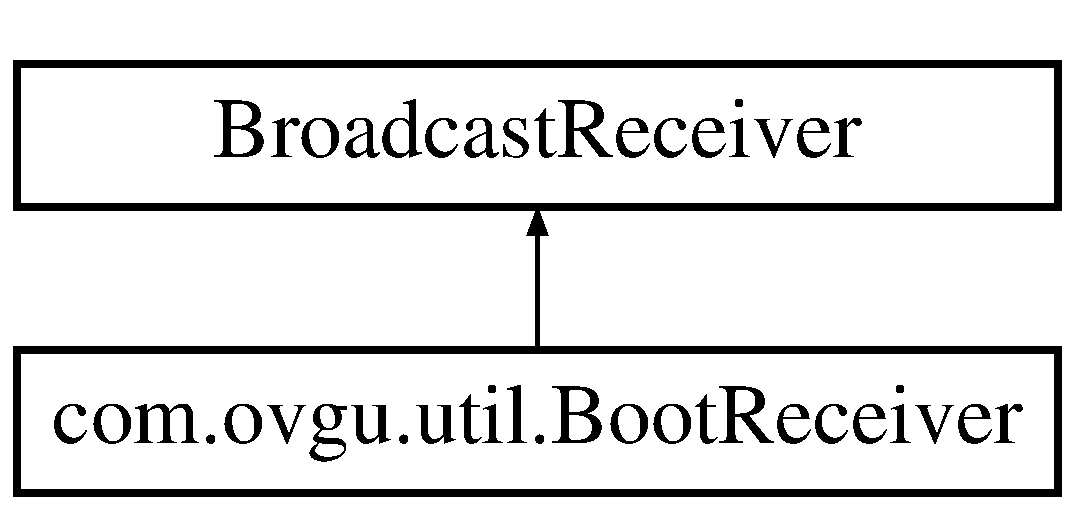
\includegraphics[height=2.000000cm]{classcom_1_1ovgu_1_1util_1_1_boot_receiver}
\end{center}
\end{figure}
\subsection*{Public Member Functions}
\begin{DoxyCompactItemize}
\item 
void \hyperlink{classcom_1_1ovgu_1_1util_1_1_boot_receiver_a13fe04fd3f5ab21b8b90e289d5ee94f1}{on\-Receive} (Context context, Intent intent)
\end{DoxyCompactItemize}


\subsection{Detailed Description}
This class gets called when the android smartphones reboots. We set the alarms as they were reset after shutting down the device \begin{DoxyAuthor}{Author}
Igor Lueckel 
\end{DoxyAuthor}


\subsection{Member Function Documentation}
\hypertarget{classcom_1_1ovgu_1_1util_1_1_boot_receiver_a13fe04fd3f5ab21b8b90e289d5ee94f1}{\index{com\-::ovgu\-::util\-::\-Boot\-Receiver@{com\-::ovgu\-::util\-::\-Boot\-Receiver}!on\-Receive@{on\-Receive}}
\index{on\-Receive@{on\-Receive}!com::ovgu::util::BootReceiver@{com\-::ovgu\-::util\-::\-Boot\-Receiver}}
\subsubsection[{on\-Receive}]{\setlength{\rightskip}{0pt plus 5cm}void com.\-ovgu.\-util.\-Boot\-Receiver.\-on\-Receive (
\begin{DoxyParamCaption}
\item[{Context}]{context, }
\item[{Intent}]{intent}
\end{DoxyParamCaption}
)}}\label{classcom_1_1ovgu_1_1util_1_1_boot_receiver_a13fe04fd3f5ab21b8b90e289d5ee94f1}


The documentation for this class was generated from the following file\-:\begin{DoxyCompactItemize}
\item 
C\-:/\-Users/\-Igor/\-Android/workspace/\-Z\-I\-M/src/com/ovgu/util/Boot\-Receiver.\-java\end{DoxyCompactItemize}

\hypertarget{classcom_1_1ovgu_1_1zim_1_1_build_config}{\section{com.\-ovgu.\-zim.\-Build\-Config Class Reference}
\label{classcom_1_1ovgu_1_1zim_1_1_build_config}\index{com.\-ovgu.\-zim.\-Build\-Config@{com.\-ovgu.\-zim.\-Build\-Config}}
}
\subsection*{Static Public Attributes}
\begin{DoxyCompactItemize}
\item 
\hypertarget{classcom_1_1ovgu_1_1zim_1_1_build_config_af24e7148bf08f4fddf4eb50a01de3c10}{static final boolean {\bfseries D\-E\-B\-U\-G} = true}\label{classcom_1_1ovgu_1_1zim_1_1_build_config_af24e7148bf08f4fddf4eb50a01de3c10}

\end{DoxyCompactItemize}


The documentation for this class was generated from the following file\-:\begin{DoxyCompactItemize}
\item 
C\-:/\-Users/\-Igor/\-Android/workspace/\-Z\-I\-M/gen/com/ovgu/zim/Build\-Config.\-java\end{DoxyCompactItemize}

\hypertarget{classcom_1_1ovgu_1_1util_1_1_c_s_v_exporter}{\section{com.\-ovgu.\-util.\-C\-S\-V\-Exporter Class Reference}
\label{classcom_1_1ovgu_1_1util_1_1_c_s_v_exporter}\index{com.\-ovgu.\-util.\-C\-S\-V\-Exporter@{com.\-ovgu.\-util.\-C\-S\-V\-Exporter}}
}
\subsection*{Public Member Functions}
\begin{DoxyCompactItemize}
\item 
void \hyperlink{classcom_1_1ovgu_1_1util_1_1_c_s_v_exporter_afb338747d41a7b01b8040dc36e17d327}{export\-As\-Csv} (Context context)
\end{DoxyCompactItemize}


\subsection{Detailed Description}
This class is a warpper for exporting datasets into a csv file in the public accessable storage \begin{DoxyAuthor}{Author}
Igor Lueckel 
\end{DoxyAuthor}


\subsection{Member Function Documentation}
\hypertarget{classcom_1_1ovgu_1_1util_1_1_c_s_v_exporter_afb338747d41a7b01b8040dc36e17d327}{\index{com\-::ovgu\-::util\-::\-C\-S\-V\-Exporter@{com\-::ovgu\-::util\-::\-C\-S\-V\-Exporter}!export\-As\-Csv@{export\-As\-Csv}}
\index{export\-As\-Csv@{export\-As\-Csv}!com::ovgu::util::CSVExporter@{com\-::ovgu\-::util\-::\-C\-S\-V\-Exporter}}
\subsubsection[{export\-As\-Csv}]{\setlength{\rightskip}{0pt plus 5cm}void com.\-ovgu.\-util.\-C\-S\-V\-Exporter.\-export\-As\-Csv (
\begin{DoxyParamCaption}
\item[{Context}]{context}
\end{DoxyParamCaption}
)}}\label{classcom_1_1ovgu_1_1util_1_1_c_s_v_exporter_afb338747d41a7b01b8040dc36e17d327}
Saves and converts all entries of the J\-S\-O\-N database into the csv format. The file named by the user I\-D is saved into a folder called \char`\"{}\-Z\-I\-M\char`\"{}. 
\begin{DoxyParams}{Parameters}
{\em context} & The current application context \\
\hline
\end{DoxyParams}


The documentation for this class was generated from the following file\-:\begin{DoxyCompactItemize}
\item 
C\-:/\-Users/\-Igor/\-Android/workspace/\-Z\-I\-M/src/com/ovgu/util/C\-S\-V\-Exporter.\-java\end{DoxyCompactItemize}

\hypertarget{classcom_1_1ovgu_1_1util_1_1_database_entry}{\section{com.\-ovgu.\-util.\-Database\-Entry Class Reference}
\label{classcom_1_1ovgu_1_1util_1_1_database_entry}\index{com.\-ovgu.\-util.\-Database\-Entry@{com.\-ovgu.\-util.\-Database\-Entry}}
}
\subsection*{Public Member Functions}
\begin{DoxyCompactItemize}
\item 
String \hyperlink{classcom_1_1ovgu_1_1util_1_1_database_entry_a53818c1011103fee08f1696039efa4b5}{get\-User\-I\-D} ()
\item 
String \hyperlink{classcom_1_1ovgu_1_1util_1_1_database_entry_ab4b670bb0adde9caea76e38c73febb0e}{get\-Date} ()
\item 
String \hyperlink{classcom_1_1ovgu_1_1util_1_1_database_entry_af7f3837d6de3ee67b7f3489340191a6c}{get\-Time} ()
\item 
String \hyperlink{classcom_1_1ovgu_1_1util_1_1_database_entry_a51863be14ac2cc7a494310b54e3da0df}{get\-Answer\-Time} ()
\item 
String \hyperlink{classcom_1_1ovgu_1_1util_1_1_database_entry_a3af262f3003fb93db15e3f752784e2de}{get\-Contacts} ()
\item 
String \hyperlink{classcom_1_1ovgu_1_1util_1_1_database_entry_ad286e4cde28731cab8012622f3cebb4f}{get\-Contact\-Time} ()
\item 
void \hyperlink{classcom_1_1ovgu_1_1util_1_1_database_entry_a023633441e5765e247eaee998e6f62a8}{set\-User\-I\-D} (String value)
\item 
void \hyperlink{classcom_1_1ovgu_1_1util_1_1_database_entry_a316eee6a35971dd7f8bb09a2e64964d7}{set\-Date} (String value)
\item 
void \hyperlink{classcom_1_1ovgu_1_1util_1_1_database_entry_a7fd9b1ec15f6381d240e9709edf0ee42}{set\-Time} (String value)
\item 
void \hyperlink{classcom_1_1ovgu_1_1util_1_1_database_entry_aafadffefd6154e5611c19990a2706ced}{set\-Answer\-Time} (String value)
\item 
void \hyperlink{classcom_1_1ovgu_1_1util_1_1_database_entry_aa603a98fdddc90e4a2150a19143a1dd3}{set\-Contacts} (String value)
\item 
void \hyperlink{classcom_1_1ovgu_1_1util_1_1_database_entry_a6e44d812319dd9c7a8dd30302f412283}{set\-Contact\-Time} (String value)
\item 
String \hyperlink{classcom_1_1ovgu_1_1util_1_1_database_entry_a12e0a8032913a9f99c44f5f287783396}{to\-C\-S\-V} ()
\end{DoxyCompactItemize}
\subsection*{Static Public Member Functions}
\begin{DoxyCompactItemize}
\item 
static String \hyperlink{classcom_1_1ovgu_1_1util_1_1_database_entry_a2cacf692bcb29a4a8af62f079f0883cb}{csv\-Header} ()
\end{DoxyCompactItemize}


\subsection{Detailed Description}
This class is intended to store temporary data from the user input. \begin{DoxyAuthor}{Author}
Igor Lueckel 
\end{DoxyAuthor}


\subsection{Member Function Documentation}
\hypertarget{classcom_1_1ovgu_1_1util_1_1_database_entry_a2cacf692bcb29a4a8af62f079f0883cb}{\index{com\-::ovgu\-::util\-::\-Database\-Entry@{com\-::ovgu\-::util\-::\-Database\-Entry}!csv\-Header@{csv\-Header}}
\index{csv\-Header@{csv\-Header}!com::ovgu::util::DatabaseEntry@{com\-::ovgu\-::util\-::\-Database\-Entry}}
\subsubsection[{csv\-Header}]{\setlength{\rightskip}{0pt plus 5cm}static String com.\-ovgu.\-util.\-Database\-Entry.\-csv\-Header (
\begin{DoxyParamCaption}
{}
\end{DoxyParamCaption}
)\hspace{0.3cm}{\ttfamily [static]}}}\label{classcom_1_1ovgu_1_1util_1_1_database_entry_a2cacf692bcb29a4a8af62f079f0883cb}
This string should be used as first line in a csv file \begin{DoxyReturn}{Returns}
Returns a header line containing all data fields 
\end{DoxyReturn}
\hypertarget{classcom_1_1ovgu_1_1util_1_1_database_entry_a51863be14ac2cc7a494310b54e3da0df}{\index{com\-::ovgu\-::util\-::\-Database\-Entry@{com\-::ovgu\-::util\-::\-Database\-Entry}!get\-Answer\-Time@{get\-Answer\-Time}}
\index{get\-Answer\-Time@{get\-Answer\-Time}!com::ovgu::util::DatabaseEntry@{com\-::ovgu\-::util\-::\-Database\-Entry}}
\subsubsection[{get\-Answer\-Time}]{\setlength{\rightskip}{0pt plus 5cm}String com.\-ovgu.\-util.\-Database\-Entry.\-get\-Answer\-Time (
\begin{DoxyParamCaption}
{}
\end{DoxyParamCaption}
)}}\label{classcom_1_1ovgu_1_1util_1_1_database_entry_a51863be14ac2cc7a494310b54e3da0df}
\begin{DoxyReturn}{Returns}
Returns the time (hh\-:mm) when the user saved the data 
\end{DoxyReturn}
\hypertarget{classcom_1_1ovgu_1_1util_1_1_database_entry_a3af262f3003fb93db15e3f752784e2de}{\index{com\-::ovgu\-::util\-::\-Database\-Entry@{com\-::ovgu\-::util\-::\-Database\-Entry}!get\-Contacts@{get\-Contacts}}
\index{get\-Contacts@{get\-Contacts}!com::ovgu::util::DatabaseEntry@{com\-::ovgu\-::util\-::\-Database\-Entry}}
\subsubsection[{get\-Contacts}]{\setlength{\rightskip}{0pt plus 5cm}String com.\-ovgu.\-util.\-Database\-Entry.\-get\-Contacts (
\begin{DoxyParamCaption}
{}
\end{DoxyParamCaption}
)}}\label{classcom_1_1ovgu_1_1util_1_1_database_entry_a3af262f3003fb93db15e3f752784e2de}
\begin{DoxyReturn}{Returns}
Returns the amount of contacts 
\end{DoxyReturn}
\hypertarget{classcom_1_1ovgu_1_1util_1_1_database_entry_ad286e4cde28731cab8012622f3cebb4f}{\index{com\-::ovgu\-::util\-::\-Database\-Entry@{com\-::ovgu\-::util\-::\-Database\-Entry}!get\-Contact\-Time@{get\-Contact\-Time}}
\index{get\-Contact\-Time@{get\-Contact\-Time}!com::ovgu::util::DatabaseEntry@{com\-::ovgu\-::util\-::\-Database\-Entry}}
\subsubsection[{get\-Contact\-Time}]{\setlength{\rightskip}{0pt plus 5cm}String com.\-ovgu.\-util.\-Database\-Entry.\-get\-Contact\-Time (
\begin{DoxyParamCaption}
{}
\end{DoxyParamCaption}
)}}\label{classcom_1_1ovgu_1_1util_1_1_database_entry_ad286e4cde28731cab8012622f3cebb4f}
\begin{DoxyReturn}{Returns}
Returns the amount of time spend with the contacts in the format hh\-:mm 
\end{DoxyReturn}
\hypertarget{classcom_1_1ovgu_1_1util_1_1_database_entry_ab4b670bb0adde9caea76e38c73febb0e}{\index{com\-::ovgu\-::util\-::\-Database\-Entry@{com\-::ovgu\-::util\-::\-Database\-Entry}!get\-Date@{get\-Date}}
\index{get\-Date@{get\-Date}!com::ovgu::util::DatabaseEntry@{com\-::ovgu\-::util\-::\-Database\-Entry}}
\subsubsection[{get\-Date}]{\setlength{\rightskip}{0pt plus 5cm}String com.\-ovgu.\-util.\-Database\-Entry.\-get\-Date (
\begin{DoxyParamCaption}
{}
\end{DoxyParamCaption}
)}}\label{classcom_1_1ovgu_1_1util_1_1_database_entry_ab4b670bb0adde9caea76e38c73febb0e}
\begin{DoxyReturn}{Returns}
Returns the alarmdate with following format\-: dd.\-mm.\-yy 
\end{DoxyReturn}
\hypertarget{classcom_1_1ovgu_1_1util_1_1_database_entry_af7f3837d6de3ee67b7f3489340191a6c}{\index{com\-::ovgu\-::util\-::\-Database\-Entry@{com\-::ovgu\-::util\-::\-Database\-Entry}!get\-Time@{get\-Time}}
\index{get\-Time@{get\-Time}!com::ovgu::util::DatabaseEntry@{com\-::ovgu\-::util\-::\-Database\-Entry}}
\subsubsection[{get\-Time}]{\setlength{\rightskip}{0pt plus 5cm}String com.\-ovgu.\-util.\-Database\-Entry.\-get\-Time (
\begin{DoxyParamCaption}
{}
\end{DoxyParamCaption}
)}}\label{classcom_1_1ovgu_1_1util_1_1_database_entry_af7f3837d6de3ee67b7f3489340191a6c}
\begin{DoxyReturn}{Returns}
Returns the alarmtime with the following format\-: hh\-:mm 
\end{DoxyReturn}
\hypertarget{classcom_1_1ovgu_1_1util_1_1_database_entry_a53818c1011103fee08f1696039efa4b5}{\index{com\-::ovgu\-::util\-::\-Database\-Entry@{com\-::ovgu\-::util\-::\-Database\-Entry}!get\-User\-I\-D@{get\-User\-I\-D}}
\index{get\-User\-I\-D@{get\-User\-I\-D}!com::ovgu::util::DatabaseEntry@{com\-::ovgu\-::util\-::\-Database\-Entry}}
\subsubsection[{get\-User\-I\-D}]{\setlength{\rightskip}{0pt plus 5cm}String com.\-ovgu.\-util.\-Database\-Entry.\-get\-User\-I\-D (
\begin{DoxyParamCaption}
{}
\end{DoxyParamCaption}
)}}\label{classcom_1_1ovgu_1_1util_1_1_database_entry_a53818c1011103fee08f1696039efa4b5}
\begin{DoxyReturn}{Returns}
Returns the User\-I\-D (Probandencode) 
\end{DoxyReturn}
\hypertarget{classcom_1_1ovgu_1_1util_1_1_database_entry_aafadffefd6154e5611c19990a2706ced}{\index{com\-::ovgu\-::util\-::\-Database\-Entry@{com\-::ovgu\-::util\-::\-Database\-Entry}!set\-Answer\-Time@{set\-Answer\-Time}}
\index{set\-Answer\-Time@{set\-Answer\-Time}!com::ovgu::util::DatabaseEntry@{com\-::ovgu\-::util\-::\-Database\-Entry}}
\subsubsection[{set\-Answer\-Time}]{\setlength{\rightskip}{0pt plus 5cm}void com.\-ovgu.\-util.\-Database\-Entry.\-set\-Answer\-Time (
\begin{DoxyParamCaption}
\item[{String}]{value}
\end{DoxyParamCaption}
)}}\label{classcom_1_1ovgu_1_1util_1_1_database_entry_aafadffefd6154e5611c19990a2706ced}
Sets delay between the actual alarm and the point of saving the data Set -\/77 if the user does not anwserd it 
\begin{DoxyParams}{Parameters}
{\em value} & String containing the amount of time spend with the contacts (hh\-:mm) \\
\hline
\end{DoxyParams}
\hypertarget{classcom_1_1ovgu_1_1util_1_1_database_entry_aa603a98fdddc90e4a2150a19143a1dd3}{\index{com\-::ovgu\-::util\-::\-Database\-Entry@{com\-::ovgu\-::util\-::\-Database\-Entry}!set\-Contacts@{set\-Contacts}}
\index{set\-Contacts@{set\-Contacts}!com::ovgu::util::DatabaseEntry@{com\-::ovgu\-::util\-::\-Database\-Entry}}
\subsubsection[{set\-Contacts}]{\setlength{\rightskip}{0pt plus 5cm}void com.\-ovgu.\-util.\-Database\-Entry.\-set\-Contacts (
\begin{DoxyParamCaption}
\item[{String}]{value}
\end{DoxyParamCaption}
)}}\label{classcom_1_1ovgu_1_1util_1_1_database_entry_aa603a98fdddc90e4a2150a19143a1dd3}
Sets the amount of contacts the participant had Set -\/77 if the user does not anwserd it 
\begin{DoxyParams}{Parameters}
{\em value} & String containing the amount of contacts \\
\hline
\end{DoxyParams}
\hypertarget{classcom_1_1ovgu_1_1util_1_1_database_entry_a6e44d812319dd9c7a8dd30302f412283}{\index{com\-::ovgu\-::util\-::\-Database\-Entry@{com\-::ovgu\-::util\-::\-Database\-Entry}!set\-Contact\-Time@{set\-Contact\-Time}}
\index{set\-Contact\-Time@{set\-Contact\-Time}!com::ovgu::util::DatabaseEntry@{com\-::ovgu\-::util\-::\-Database\-Entry}}
\subsubsection[{set\-Contact\-Time}]{\setlength{\rightskip}{0pt plus 5cm}void com.\-ovgu.\-util.\-Database\-Entry.\-set\-Contact\-Time (
\begin{DoxyParamCaption}
\item[{String}]{value}
\end{DoxyParamCaption}
)}}\label{classcom_1_1ovgu_1_1util_1_1_database_entry_a6e44d812319dd9c7a8dd30302f412283}
Sets the amount of minutes the participant spend with the contacts Set -\/77 if the user does not anwserd it 
\begin{DoxyParams}{Parameters}
{\em value} & String containing the amount of time spend with the contacts (format hh\-:mm) \\
\hline
\end{DoxyParams}
\hypertarget{classcom_1_1ovgu_1_1util_1_1_database_entry_a316eee6a35971dd7f8bb09a2e64964d7}{\index{com\-::ovgu\-::util\-::\-Database\-Entry@{com\-::ovgu\-::util\-::\-Database\-Entry}!set\-Date@{set\-Date}}
\index{set\-Date@{set\-Date}!com::ovgu::util::DatabaseEntry@{com\-::ovgu\-::util\-::\-Database\-Entry}}
\subsubsection[{set\-Date}]{\setlength{\rightskip}{0pt plus 5cm}void com.\-ovgu.\-util.\-Database\-Entry.\-set\-Date (
\begin{DoxyParamCaption}
\item[{String}]{value}
\end{DoxyParamCaption}
)}}\label{classcom_1_1ovgu_1_1util_1_1_database_entry_a316eee6a35971dd7f8bb09a2e64964d7}
Sets the alarmdate 
\begin{DoxyParams}{Parameters}
{\em value} & String containing the alarmdate with the format\-: dd.\-mm.\-yy \\
\hline
\end{DoxyParams}
\hypertarget{classcom_1_1ovgu_1_1util_1_1_database_entry_a7fd9b1ec15f6381d240e9709edf0ee42}{\index{com\-::ovgu\-::util\-::\-Database\-Entry@{com\-::ovgu\-::util\-::\-Database\-Entry}!set\-Time@{set\-Time}}
\index{set\-Time@{set\-Time}!com::ovgu::util::DatabaseEntry@{com\-::ovgu\-::util\-::\-Database\-Entry}}
\subsubsection[{set\-Time}]{\setlength{\rightskip}{0pt plus 5cm}void com.\-ovgu.\-util.\-Database\-Entry.\-set\-Time (
\begin{DoxyParamCaption}
\item[{String}]{value}
\end{DoxyParamCaption}
)}}\label{classcom_1_1ovgu_1_1util_1_1_database_entry_a7fd9b1ec15f6381d240e9709edf0ee42}
Sets the alarmtime 
\begin{DoxyParams}{Parameters}
{\em value} & String containing the alarmtime with the format\-: hh\-:mm \\
\hline
\end{DoxyParams}
\hypertarget{classcom_1_1ovgu_1_1util_1_1_database_entry_a023633441e5765e247eaee998e6f62a8}{\index{com\-::ovgu\-::util\-::\-Database\-Entry@{com\-::ovgu\-::util\-::\-Database\-Entry}!set\-User\-I\-D@{set\-User\-I\-D}}
\index{set\-User\-I\-D@{set\-User\-I\-D}!com::ovgu::util::DatabaseEntry@{com\-::ovgu\-::util\-::\-Database\-Entry}}
\subsubsection[{set\-User\-I\-D}]{\setlength{\rightskip}{0pt plus 5cm}void com.\-ovgu.\-util.\-Database\-Entry.\-set\-User\-I\-D (
\begin{DoxyParamCaption}
\item[{String}]{value}
\end{DoxyParamCaption}
)}}\label{classcom_1_1ovgu_1_1util_1_1_database_entry_a023633441e5765e247eaee998e6f62a8}
Sets a new User\-I\-D (Probandencode) 
\begin{DoxyParams}{Parameters}
{\em value} & String containing the new User\-I\-D \\
\hline
\end{DoxyParams}
\hypertarget{classcom_1_1ovgu_1_1util_1_1_database_entry_a12e0a8032913a9f99c44f5f287783396}{\index{com\-::ovgu\-::util\-::\-Database\-Entry@{com\-::ovgu\-::util\-::\-Database\-Entry}!to\-C\-S\-V@{to\-C\-S\-V}}
\index{to\-C\-S\-V@{to\-C\-S\-V}!com::ovgu::util::DatabaseEntry@{com\-::ovgu\-::util\-::\-Database\-Entry}}
\subsubsection[{to\-C\-S\-V}]{\setlength{\rightskip}{0pt plus 5cm}String com.\-ovgu.\-util.\-Database\-Entry.\-to\-C\-S\-V (
\begin{DoxyParamCaption}
{}
\end{DoxyParamCaption}
)}}\label{classcom_1_1ovgu_1_1util_1_1_database_entry_a12e0a8032913a9f99c44f5f287783396}
Use this String in the csv exporter to convert the object into an csv-\/row \begin{DoxyReturn}{Returns}
Returns a line containing all values in csv-\/format 
\end{DoxyReturn}

\begin{DoxyExceptions}{Exceptions}
{\em Parse\-Exception} & Date or time is in the wrong format \\
\hline
\end{DoxyExceptions}


The documentation for this class was generated from the following file\-:\begin{DoxyCompactItemize}
\item 
C\-:/\-Users/\-Igor/\-Android/workspace/\-Z\-I\-M/src/com/ovgu/util/Database\-Entry.\-java\end{DoxyCompactItemize}

\hypertarget{classcom_1_1ovgu_1_1jsondb_1_1_d_b_entry_deserializer}{\section{com.\-ovgu.\-jsondb.\-D\-B\-Entry\-Deserializer Class Reference}
\label{classcom_1_1ovgu_1_1jsondb_1_1_d_b_entry_deserializer}\index{com.\-ovgu.\-jsondb.\-D\-B\-Entry\-Deserializer@{com.\-ovgu.\-jsondb.\-D\-B\-Entry\-Deserializer}}
}
Inheritance diagram for com.\-ovgu.\-jsondb.\-D\-B\-Entry\-Deserializer\-:\begin{figure}[H]
\begin{center}
\leavevmode
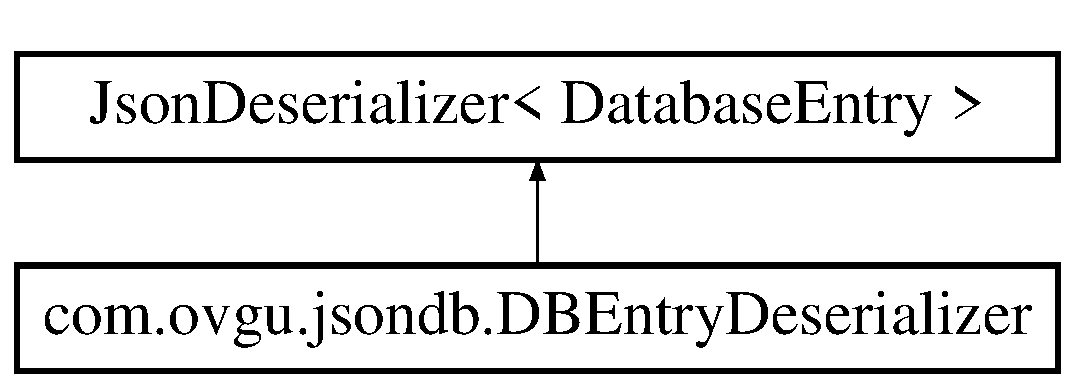
\includegraphics[height=2.000000cm]{classcom_1_1ovgu_1_1jsondb_1_1_d_b_entry_deserializer}
\end{center}
\end{figure}
\subsection*{Public Member Functions}
\begin{DoxyCompactItemize}
\item 
\hypertarget{classcom_1_1ovgu_1_1jsondb_1_1_d_b_entry_deserializer_ae7ecca25a610bfa3faa821f3d9e96513}{\hyperlink{classcom_1_1ovgu_1_1util_1_1_database_entry}{Database\-Entry} {\bfseries deserialize} (Json\-Element json, Type type\-Of\-T, Json\-Deserialization\-Context context)  throws Json\-Parse\-Exception }\label{classcom_1_1ovgu_1_1jsondb_1_1_d_b_entry_deserializer_ae7ecca25a610bfa3faa821f3d9e96513}

\end{DoxyCompactItemize}


\subsection{Detailed Description}
This class hepls to deserialize the json object to an \hyperlink{}{Database\-Entry} \begin{DoxyAuthor}{Author}
Igor Lueckel 
\end{DoxyAuthor}


The documentation for this class was generated from the following file\-:\begin{DoxyCompactItemize}
\item 
C\-:/\-Users/\-Igor/\-Android/workspace/\-Z\-I\-M/src/com/ovgu/jsondb/D\-B\-Entry\-Deserializer.\-java\end{DoxyCompactItemize}

\hypertarget{classcom_1_1ovgu_1_1jsondb_1_1_d_b_entry_serializer}{\section{com.\-ovgu.\-jsondb.\-D\-B\-Entry\-Serializer Class Reference}
\label{classcom_1_1ovgu_1_1jsondb_1_1_d_b_entry_serializer}\index{com.\-ovgu.\-jsondb.\-D\-B\-Entry\-Serializer@{com.\-ovgu.\-jsondb.\-D\-B\-Entry\-Serializer}}
}
Inheritance diagram for com.\-ovgu.\-jsondb.\-D\-B\-Entry\-Serializer\-:\begin{figure}[H]
\begin{center}
\leavevmode
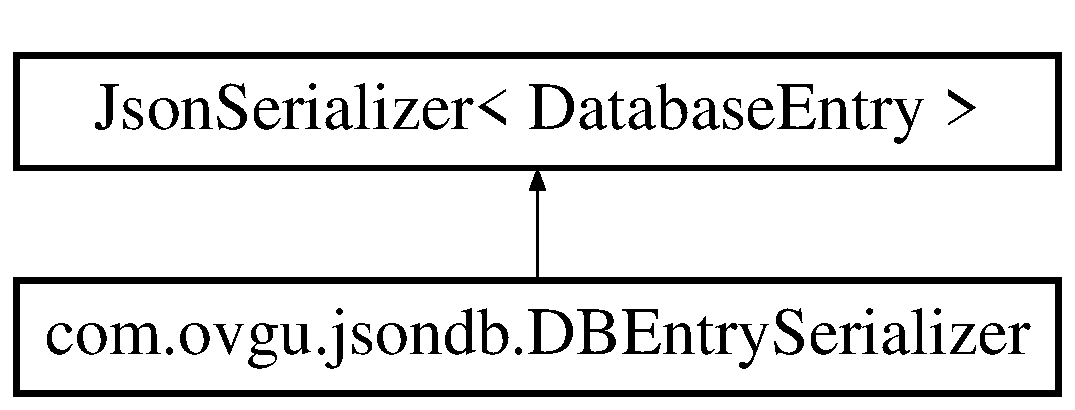
\includegraphics[height=2.000000cm]{classcom_1_1ovgu_1_1jsondb_1_1_d_b_entry_serializer}
\end{center}
\end{figure}
\subsection*{Public Member Functions}
\begin{DoxyCompactItemize}
\item 
Json\-Element \hyperlink{classcom_1_1ovgu_1_1jsondb_1_1_d_b_entry_serializer_aa490898a0cd2193b24784ca83a64e50c}{serialize} (\hyperlink{classcom_1_1ovgu_1_1util_1_1_database_entry}{Database\-Entry} src, Type type\-Of\-Src, Json\-Serialization\-Context context)
\end{DoxyCompactItemize}


\subsection{Detailed Description}
This class helps to serialize objects of \hyperlink{}{Database\-Entry} \begin{DoxyAuthor}{Author}
Igor Lueckel 
\end{DoxyAuthor}


\subsection{Member Function Documentation}
\hypertarget{classcom_1_1ovgu_1_1jsondb_1_1_d_b_entry_serializer_aa490898a0cd2193b24784ca83a64e50c}{\index{com\-::ovgu\-::jsondb\-::\-D\-B\-Entry\-Serializer@{com\-::ovgu\-::jsondb\-::\-D\-B\-Entry\-Serializer}!serialize@{serialize}}
\index{serialize@{serialize}!com::ovgu::jsondb::DBEntrySerializer@{com\-::ovgu\-::jsondb\-::\-D\-B\-Entry\-Serializer}}
\subsubsection[{serialize}]{\setlength{\rightskip}{0pt plus 5cm}Json\-Element com.\-ovgu.\-jsondb.\-D\-B\-Entry\-Serializer.\-serialize (
\begin{DoxyParamCaption}
\item[{{\bf Database\-Entry}}]{src, }
\item[{Type}]{type\-Of\-Src, }
\item[{Json\-Serialization\-Context}]{context}
\end{DoxyParamCaption}
)}}\label{classcom_1_1ovgu_1_1jsondb_1_1_d_b_entry_serializer_aa490898a0cd2193b24784ca83a64e50c}


The documentation for this class was generated from the following file\-:\begin{DoxyCompactItemize}
\item 
C\-:/\-Users/\-Igor/\-Android/workspace/\-Z\-I\-M/src/com/ovgu/jsondb/D\-B\-Entry\-Serializer.\-java\end{DoxyCompactItemize}

\hypertarget{classcom_1_1ovgu_1_1jsondb_1_1_j_s_o_n_connector}{\section{com.\-ovgu.\-jsondb.\-J\-S\-O\-N\-Connector Class Reference}
\label{classcom_1_1ovgu_1_1jsondb_1_1_j_s_o_n_connector}\index{com.\-ovgu.\-jsondb.\-J\-S\-O\-N\-Connector@{com.\-ovgu.\-jsondb.\-J\-S\-O\-N\-Connector}}
}
\subsection*{Static Public Member Functions}
\begin{DoxyCompactItemize}
\item 
static void \hyperlink{classcom_1_1ovgu_1_1jsondb_1_1_j_s_o_n_connector_a112f195b08f25e352c3148c9c930e920}{add\-Entry} (\hyperlink{classcom_1_1ovgu_1_1util_1_1_database_entry}{Database\-Entry} entry, Context ctx)
\item 
static List$<$ \hyperlink{classcom_1_1ovgu_1_1util_1_1_database_entry}{Database\-Entry} $>$ \hyperlink{classcom_1_1ovgu_1_1jsondb_1_1_j_s_o_n_connector_af5b2897760749ce7d5e7ee5a7e7617f7}{get\-All\-Entries} (Context ctx)
\item 
static void \hyperlink{classcom_1_1ovgu_1_1jsondb_1_1_j_s_o_n_connector_abd4d4fba31c513848a85b22bce65fdeb}{delete\-Entries} (Context ctx)
\end{DoxyCompactItemize}


\subsection{Detailed Description}
This class is wrapper to store items of \hyperlink{}{Database\-Entry} to an local database \begin{DoxyAuthor}{Author}
Igor Lueckel 
\end{DoxyAuthor}


\subsection{Member Function Documentation}
\hypertarget{classcom_1_1ovgu_1_1jsondb_1_1_j_s_o_n_connector_a112f195b08f25e352c3148c9c930e920}{\index{com\-::ovgu\-::jsondb\-::\-J\-S\-O\-N\-Connector@{com\-::ovgu\-::jsondb\-::\-J\-S\-O\-N\-Connector}!add\-Entry@{add\-Entry}}
\index{add\-Entry@{add\-Entry}!com::ovgu::jsondb::JSONConnector@{com\-::ovgu\-::jsondb\-::\-J\-S\-O\-N\-Connector}}
\subsubsection[{add\-Entry}]{\setlength{\rightskip}{0pt plus 5cm}static void com.\-ovgu.\-jsondb.\-J\-S\-O\-N\-Connector.\-add\-Entry (
\begin{DoxyParamCaption}
\item[{{\bf Database\-Entry}}]{entry, }
\item[{Context}]{ctx}
\end{DoxyParamCaption}
)\hspace{0.3cm}{\ttfamily [static]}}}\label{classcom_1_1ovgu_1_1jsondb_1_1_j_s_o_n_connector_a112f195b08f25e352c3148c9c930e920}
Adds an entry to the local json file 
\begin{DoxyParams}{Parameters}
{\em entry} & The Database\-Entry with data from the user \\
\hline
\end{DoxyParams}

\begin{DoxyExceptions}{Exceptions}
{\em I\-O\-Exception} & \\
\hline
\end{DoxyExceptions}
\hypertarget{classcom_1_1ovgu_1_1jsondb_1_1_j_s_o_n_connector_abd4d4fba31c513848a85b22bce65fdeb}{\index{com\-::ovgu\-::jsondb\-::\-J\-S\-O\-N\-Connector@{com\-::ovgu\-::jsondb\-::\-J\-S\-O\-N\-Connector}!delete\-Entries@{delete\-Entries}}
\index{delete\-Entries@{delete\-Entries}!com::ovgu::jsondb::JSONConnector@{com\-::ovgu\-::jsondb\-::\-J\-S\-O\-N\-Connector}}
\subsubsection[{delete\-Entries}]{\setlength{\rightskip}{0pt plus 5cm}static void com.\-ovgu.\-jsondb.\-J\-S\-O\-N\-Connector.\-delete\-Entries (
\begin{DoxyParamCaption}
\item[{Context}]{ctx}
\end{DoxyParamCaption}
)\hspace{0.3cm}{\ttfamily [static]}}}\label{classcom_1_1ovgu_1_1jsondb_1_1_j_s_o_n_connector_abd4d4fba31c513848a85b22bce65fdeb}
This methode deletes the local json files. All datas saved in it will be lost \hypertarget{classcom_1_1ovgu_1_1jsondb_1_1_j_s_o_n_connector_af5b2897760749ce7d5e7ee5a7e7617f7}{\index{com\-::ovgu\-::jsondb\-::\-J\-S\-O\-N\-Connector@{com\-::ovgu\-::jsondb\-::\-J\-S\-O\-N\-Connector}!get\-All\-Entries@{get\-All\-Entries}}
\index{get\-All\-Entries@{get\-All\-Entries}!com::ovgu::jsondb::JSONConnector@{com\-::ovgu\-::jsondb\-::\-J\-S\-O\-N\-Connector}}
\subsubsection[{get\-All\-Entries}]{\setlength{\rightskip}{0pt plus 5cm}static List$<${\bf Database\-Entry}$>$ com.\-ovgu.\-jsondb.\-J\-S\-O\-N\-Connector.\-get\-All\-Entries (
\begin{DoxyParamCaption}
\item[{Context}]{ctx}
\end{DoxyParamCaption}
)\hspace{0.3cm}{\ttfamily [static]}}}\label{classcom_1_1ovgu_1_1jsondb_1_1_j_s_o_n_connector_af5b2897760749ce7d5e7ee5a7e7617f7}
This function reads the local json file and converts all json objects into java objects. If there are no saved datas the function returns an empty list \begin{DoxyReturn}{Returns}
Returns a list of all entries saved on the phone 
\end{DoxyReturn}

\begin{DoxyParams}{Parameters}
{\em ctx} & The current application context \\
\hline
\end{DoxyParams}


The documentation for this class was generated from the following file\-:\begin{DoxyCompactItemize}
\item 
C\-:/\-Users/\-Igor/\-Android/workspace/\-Z\-I\-M/src/com/ovgu/jsondb/J\-S\-O\-N\-Connector.\-java\end{DoxyCompactItemize}

\hypertarget{classcom_1_1ovgu_1_1zim_1_1_j_s_o_n_test}{\section{com.\-ovgu.\-zim.\-J\-S\-O\-N\-Test Class Reference}
\label{classcom_1_1ovgu_1_1zim_1_1_j_s_o_n_test}\index{com.\-ovgu.\-zim.\-J\-S\-O\-N\-Test@{com.\-ovgu.\-zim.\-J\-S\-O\-N\-Test}}
}
\subsection*{Public Member Functions}
\begin{DoxyCompactItemize}
\item 
\hypertarget{classcom_1_1ovgu_1_1zim_1_1_j_s_o_n_test_a2e38804d49ebfe4b796e9c066a98fd03}{void {\bfseries set\-Up} ()  throws Exception }\label{classcom_1_1ovgu_1_1zim_1_1_j_s_o_n_test_a2e38804d49ebfe4b796e9c066a98fd03}

\item 
\hypertarget{classcom_1_1ovgu_1_1zim_1_1_j_s_o_n_test_a3f902b96830e6f01aeac01f3d0baad7c}{void {\bfseries Test\-For\-Empty\-Database} ()  throws Exception }\label{classcom_1_1ovgu_1_1zim_1_1_j_s_o_n_test_a3f902b96830e6f01aeac01f3d0baad7c}

\item 
\hypertarget{classcom_1_1ovgu_1_1zim_1_1_j_s_o_n_test_abfb65d4c2a54c558cc61e8fc959f2ae4}{void {\bfseries Add\-Single\-Entry} ()  throws Exception }\label{classcom_1_1ovgu_1_1zim_1_1_j_s_o_n_test_abfb65d4c2a54c558cc61e8fc959f2ae4}

\item 
\hypertarget{classcom_1_1ovgu_1_1zim_1_1_j_s_o_n_test_a2df6d842c388f5c59ad398ec9b0e3c65}{void {\bfseries Check\-Single\-Entry} ()  throws Exception }\label{classcom_1_1ovgu_1_1zim_1_1_j_s_o_n_test_a2df6d842c388f5c59ad398ec9b0e3c65}

\end{DoxyCompactItemize}


The documentation for this class was generated from the following file\-:\begin{DoxyCompactItemize}
\item 
C\-:/\-Users/\-Igor/\-Android/workspace/\-Z\-I\-M/test/com/ovgu/zim/J\-S\-O\-N\-Test.\-java\end{DoxyCompactItemize}

\hypertarget{classcom_1_1ovgu_1_1zim_1_1_main_activity}{\section{com.\-ovgu.\-zim.\-Main\-Activity Class Reference}
\label{classcom_1_1ovgu_1_1zim_1_1_main_activity}\index{com.\-ovgu.\-zim.\-Main\-Activity@{com.\-ovgu.\-zim.\-Main\-Activity}}
}
Inheritance diagram for com.\-ovgu.\-zim.\-Main\-Activity\-:\begin{figure}[H]
\begin{center}
\leavevmode
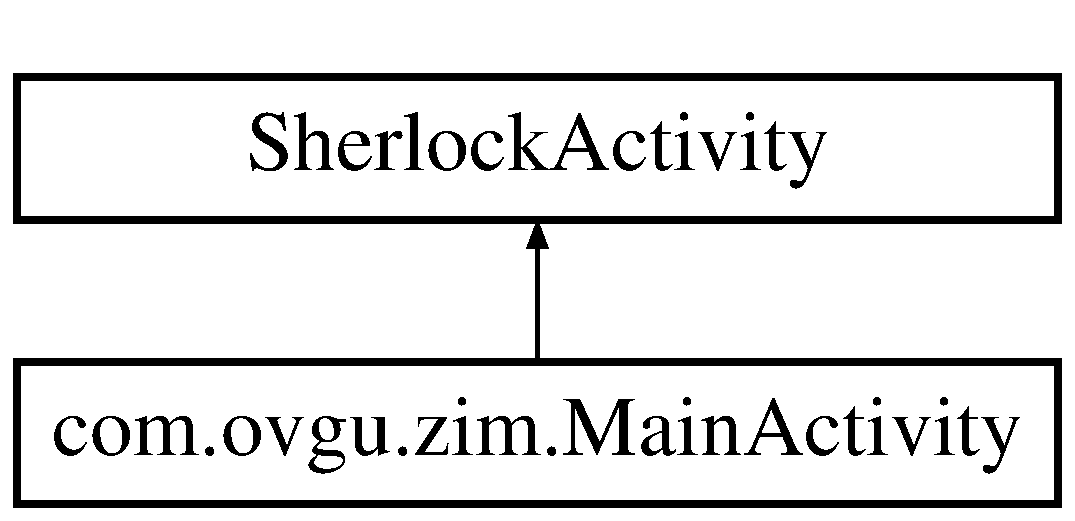
\includegraphics[height=2.000000cm]{classcom_1_1ovgu_1_1zim_1_1_main_activity}
\end{center}
\end{figure}
\subsection*{Public Member Functions}
\begin{DoxyCompactItemize}
\item 
\hypertarget{classcom_1_1ovgu_1_1zim_1_1_main_activity_ac798f4f737491eeb662eadbb28997e8e}{boolean {\bfseries on\-Create\-Options\-Menu} (Menu menu)}\label{classcom_1_1ovgu_1_1zim_1_1_main_activity_ac798f4f737491eeb662eadbb28997e8e}

\item 
void \hyperlink{classcom_1_1ovgu_1_1zim_1_1_main_activity_aabd114a80ae210faa283375f2e6bc7de}{open\-Preferences} (View view)
\item 
void \hyperlink{classcom_1_1ovgu_1_1zim_1_1_main_activity_afc4cfd60a7a114671805f0179db2eb34}{wipe\-Data} (View view)
\item 
\hypertarget{classcom_1_1ovgu_1_1zim_1_1_main_activity_ad547d8a3800ae159dffdc697ef2474da}{void {\bfseries export\-To\-C\-S\-V} (View view)}\label{classcom_1_1ovgu_1_1zim_1_1_main_activity_ad547d8a3800ae159dffdc697ef2474da}

\end{DoxyCompactItemize}
\subsection*{Protected Member Functions}
\begin{DoxyCompactItemize}
\item 
\hypertarget{classcom_1_1ovgu_1_1zim_1_1_main_activity_aef946129355d6b0aae9ceb83eb072878}{void {\bfseries on\-Create} (Bundle saved\-Instance\-State)}\label{classcom_1_1ovgu_1_1zim_1_1_main_activity_aef946129355d6b0aae9ceb83eb072878}

\item 
\hypertarget{classcom_1_1ovgu_1_1zim_1_1_main_activity_a32b82a2996c3aae5312f07f54cb4226c}{void {\bfseries on\-Pause} ()}\label{classcom_1_1ovgu_1_1zim_1_1_main_activity_a32b82a2996c3aae5312f07f54cb4226c}

\item 
\hypertarget{classcom_1_1ovgu_1_1zim_1_1_main_activity_a4d9b6d96d16d56f7c1bf1d9c8ea2f348}{void {\bfseries on\-Resume} ()}\label{classcom_1_1ovgu_1_1zim_1_1_main_activity_a4d9b6d96d16d56f7c1bf1d9c8ea2f348}

\item 
\hypertarget{classcom_1_1ovgu_1_1zim_1_1_main_activity_aa4f0e30996ad68faa4caf8785972129e}{void {\bfseries on\-Destroy} ()}\label{classcom_1_1ovgu_1_1zim_1_1_main_activity_aa4f0e30996ad68faa4caf8785972129e}

\end{DoxyCompactItemize}


\subsection{Detailed Description}
The \hyperlink{classcom_1_1ovgu_1_1zim_1_1_main_activity}{Main\-Activity} is the entrypoint of the app. The user can see the next alarm time, change preferences, export data as csv and wipe the app. \begin{DoxyAuthor}{Author}
Igor Lueckel 
\end{DoxyAuthor}


\subsection{Member Function Documentation}
\hypertarget{classcom_1_1ovgu_1_1zim_1_1_main_activity_aabd114a80ae210faa283375f2e6bc7de}{\index{com\-::ovgu\-::zim\-::\-Main\-Activity@{com\-::ovgu\-::zim\-::\-Main\-Activity}!open\-Preferences@{open\-Preferences}}
\index{open\-Preferences@{open\-Preferences}!com::ovgu::zim::MainActivity@{com\-::ovgu\-::zim\-::\-Main\-Activity}}
\subsubsection[{open\-Preferences}]{\setlength{\rightskip}{0pt plus 5cm}void com.\-ovgu.\-zim.\-Main\-Activity.\-open\-Preferences (
\begin{DoxyParamCaption}
\item[{View}]{view}
\end{DoxyParamCaption}
)}}\label{classcom_1_1ovgu_1_1zim_1_1_main_activity_aabd114a80ae210faa283375f2e6bc7de}
Starts a new activity with the preference screen \hypertarget{classcom_1_1ovgu_1_1zim_1_1_main_activity_afc4cfd60a7a114671805f0179db2eb34}{\index{com\-::ovgu\-::zim\-::\-Main\-Activity@{com\-::ovgu\-::zim\-::\-Main\-Activity}!wipe\-Data@{wipe\-Data}}
\index{wipe\-Data@{wipe\-Data}!com::ovgu::zim::MainActivity@{com\-::ovgu\-::zim\-::\-Main\-Activity}}
\subsubsection[{wipe\-Data}]{\setlength{\rightskip}{0pt plus 5cm}void com.\-ovgu.\-zim.\-Main\-Activity.\-wipe\-Data (
\begin{DoxyParamCaption}
\item[{View}]{view}
\end{DoxyParamCaption}
)}}\label{classcom_1_1ovgu_1_1zim_1_1_main_activity_afc4cfd60a7a114671805f0179db2eb34}
Shows an dialoge with password box. If the password is correct, wipe\-Data() gets called. Else a toast is shown. 
\begin{DoxyParams}{Parameters}
{\em view} & \\
\hline
\end{DoxyParams}


The documentation for this class was generated from the following file\-:\begin{DoxyCompactItemize}
\item 
C\-:/\-Users/\-Igor/\-Android/workspace/\-Z\-I\-M/src/com/ovgu/zim/Main\-Activity.\-java\end{DoxyCompactItemize}

\hypertarget{classcom_1_1ovgu_1_1zim_1_1_main_activity_test}{\section{com.\-ovgu.\-zim.\-Main\-Activity\-Test Class Reference}
\label{classcom_1_1ovgu_1_1zim_1_1_main_activity_test}\index{com.\-ovgu.\-zim.\-Main\-Activity\-Test@{com.\-ovgu.\-zim.\-Main\-Activity\-Test}}
}
\subsection*{Public Member Functions}
\begin{DoxyCompactItemize}
\item 
\hypertarget{classcom_1_1ovgu_1_1zim_1_1_main_activity_test_ab969cb6c01cc9b2bcf8a856bf6528ad2}{void {\bfseries set\-Up} ()  throws Exception }\label{classcom_1_1ovgu_1_1zim_1_1_main_activity_test_ab969cb6c01cc9b2bcf8a856bf6528ad2}

\item 
\hypertarget{classcom_1_1ovgu_1_1zim_1_1_main_activity_test_a0b1194057c307417c06197c1deeda288}{void {\bfseries should\-Show\-No\-Alarm\-Set\-Text} ()  throws Exception }\label{classcom_1_1ovgu_1_1zim_1_1_main_activity_test_a0b1194057c307417c06197c1deeda288}

\item 
\hypertarget{classcom_1_1ovgu_1_1zim_1_1_main_activity_test_aef96db85384591755820a3705a78501b}{void {\bfseries should\-Open\-Preference\-Activity} ()  throws Exception }\label{classcom_1_1ovgu_1_1zim_1_1_main_activity_test_aef96db85384591755820a3705a78501b}

\end{DoxyCompactItemize}


The documentation for this class was generated from the following file\-:\begin{DoxyCompactItemize}
\item 
C\-:/\-Users/\-Igor/\-Android/workspace/\-Z\-I\-M/test/com/ovgu/zim/Main\-Activity\-Test.\-java\end{DoxyCompactItemize}

\hypertarget{classcom_1_1ovgu_1_1zim_1_1_preference_activity}{\section{com.\-ovgu.\-zim.\-Preference\-Activity Class Reference}
\label{classcom_1_1ovgu_1_1zim_1_1_preference_activity}\index{com.\-ovgu.\-zim.\-Preference\-Activity@{com.\-ovgu.\-zim.\-Preference\-Activity}}
}
Inheritance diagram for com.\-ovgu.\-zim.\-Preference\-Activity\-:\begin{figure}[H]
\begin{center}
\leavevmode
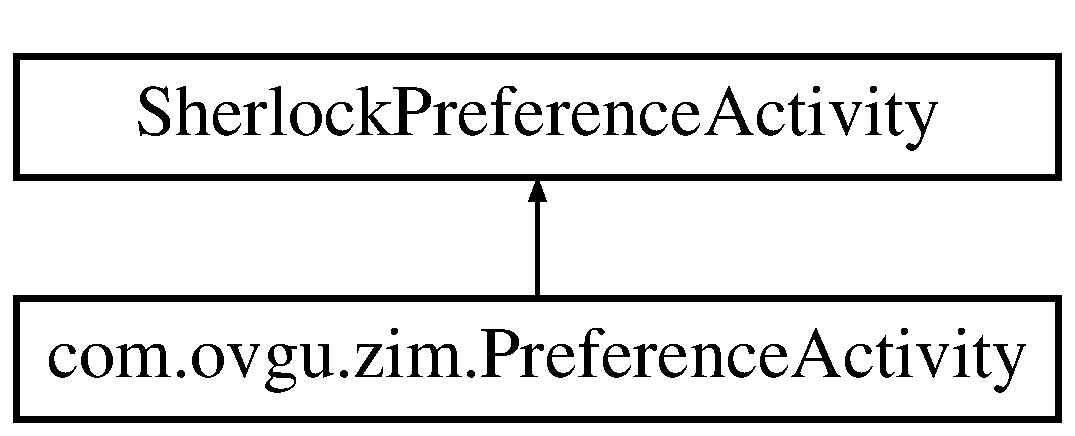
\includegraphics[height=2.000000cm]{classcom_1_1ovgu_1_1zim_1_1_preference_activity}
\end{center}
\end{figure}
\subsection*{Public Member Functions}
\begin{DoxyCompactItemize}
\item 
boolean \hyperlink{classcom_1_1ovgu_1_1zim_1_1_preference_activity_ae5d99d5ceb32fbe5e4cab59efde473df}{on\-Create\-Options\-Menu} (Menu menu)
\item 
boolean \hyperlink{classcom_1_1ovgu_1_1zim_1_1_preference_activity_a74ecec5dcb044b284cce87facb19159b}{on\-Options\-Item\-Selected} (Menu\-Item item)
\item 
void \hyperlink{classcom_1_1ovgu_1_1zim_1_1_preference_activity_a3fb88c298fd239ae6d86d0b22ee1bbc7}{on\-Back\-Pressed} ()
\end{DoxyCompactItemize}
\subsection*{Protected Member Functions}
\begin{DoxyCompactItemize}
\item 
\hypertarget{classcom_1_1ovgu_1_1zim_1_1_preference_activity_a9a9687205d6aa88d88e3f555b40d0b65}{void {\bfseries on\-Create} (Bundle saved\-Instance\-State)}\label{classcom_1_1ovgu_1_1zim_1_1_preference_activity_a9a9687205d6aa88d88e3f555b40d0b65}

\end{DoxyCompactItemize}


\subsection{Detailed Description}
Within the \hyperlink{classcom_1_1ovgu_1_1zim_1_1_preference_activity}{Preference\-Activity} the user can change alarmtimes and alarmtypes \begin{DoxyAuthor}{Author}
Igor Lueckel 
\end{DoxyAuthor}


\subsection{Member Function Documentation}
\hypertarget{classcom_1_1ovgu_1_1zim_1_1_preference_activity_a3fb88c298fd239ae6d86d0b22ee1bbc7}{\index{com\-::ovgu\-::zim\-::\-Preference\-Activity@{com\-::ovgu\-::zim\-::\-Preference\-Activity}!on\-Back\-Pressed@{on\-Back\-Pressed}}
\index{on\-Back\-Pressed@{on\-Back\-Pressed}!com::ovgu::zim::PreferenceActivity@{com\-::ovgu\-::zim\-::\-Preference\-Activity}}
\subsubsection[{on\-Back\-Pressed}]{\setlength{\rightskip}{0pt plus 5cm}void com.\-ovgu.\-zim.\-Preference\-Activity.\-on\-Back\-Pressed (
\begin{DoxyParamCaption}
{}
\end{DoxyParamCaption}
)}}\label{classcom_1_1ovgu_1_1zim_1_1_preference_activity_a3fb88c298fd239ae6d86d0b22ee1bbc7}
\hypertarget{classcom_1_1ovgu_1_1zim_1_1_preference_activity_ae5d99d5ceb32fbe5e4cab59efde473df}{\index{com\-::ovgu\-::zim\-::\-Preference\-Activity@{com\-::ovgu\-::zim\-::\-Preference\-Activity}!on\-Create\-Options\-Menu@{on\-Create\-Options\-Menu}}
\index{on\-Create\-Options\-Menu@{on\-Create\-Options\-Menu}!com::ovgu::zim::PreferenceActivity@{com\-::ovgu\-::zim\-::\-Preference\-Activity}}
\subsubsection[{on\-Create\-Options\-Menu}]{\setlength{\rightskip}{0pt plus 5cm}boolean com.\-ovgu.\-zim.\-Preference\-Activity.\-on\-Create\-Options\-Menu (
\begin{DoxyParamCaption}
\item[{Menu}]{menu}
\end{DoxyParamCaption}
)}}\label{classcom_1_1ovgu_1_1zim_1_1_preference_activity_ae5d99d5ceb32fbe5e4cab59efde473df}
\hypertarget{classcom_1_1ovgu_1_1zim_1_1_preference_activity_a74ecec5dcb044b284cce87facb19159b}{\index{com\-::ovgu\-::zim\-::\-Preference\-Activity@{com\-::ovgu\-::zim\-::\-Preference\-Activity}!on\-Options\-Item\-Selected@{on\-Options\-Item\-Selected}}
\index{on\-Options\-Item\-Selected@{on\-Options\-Item\-Selected}!com::ovgu::zim::PreferenceActivity@{com\-::ovgu\-::zim\-::\-Preference\-Activity}}
\subsubsection[{on\-Options\-Item\-Selected}]{\setlength{\rightskip}{0pt plus 5cm}boolean com.\-ovgu.\-zim.\-Preference\-Activity.\-on\-Options\-Item\-Selected (
\begin{DoxyParamCaption}
\item[{Menu\-Item}]{item}
\end{DoxyParamCaption}
)}}\label{classcom_1_1ovgu_1_1zim_1_1_preference_activity_a74ecec5dcb044b284cce87facb19159b}


The documentation for this class was generated from the following file\-:\begin{DoxyCompactItemize}
\item 
C\-:/\-Users/\-Igor/\-Android/workspace/\-Z\-I\-M/src/com/ovgu/zim/Preference\-Activity.\-java\end{DoxyCompactItemize}

\hypertarget{classcom_1_1ovgu_1_1zim_1_1_preference_activity_test}{\section{com.\-ovgu.\-zim.\-Preference\-Activity\-Test Class Reference}
\label{classcom_1_1ovgu_1_1zim_1_1_preference_activity_test}\index{com.\-ovgu.\-zim.\-Preference\-Activity\-Test@{com.\-ovgu.\-zim.\-Preference\-Activity\-Test}}
}
\subsection*{Public Member Functions}
\begin{DoxyCompactItemize}
\item 
\hypertarget{classcom_1_1ovgu_1_1zim_1_1_preference_activity_test_a8ba5cfaab3ea11a8e7b5cb4f6a84238c}{void {\bfseries set\-Up} ()  throws Exception }\label{classcom_1_1ovgu_1_1zim_1_1_preference_activity_test_a8ba5cfaab3ea11a8e7b5cb4f6a84238c}

\item 
\hypertarget{classcom_1_1ovgu_1_1zim_1_1_preference_activity_test_a405be06b8a689ea040a9781a329c6379}{void {\bfseries should\-Show\-Minus\-One} ()  throws Exception }\label{classcom_1_1ovgu_1_1zim_1_1_preference_activity_test_a405be06b8a689ea040a9781a329c6379}

\end{DoxyCompactItemize}


The documentation for this class was generated from the following file\-:\begin{DoxyCompactItemize}
\item 
C\-:/\-Users/\-Igor/\-Android/workspace/\-Z\-I\-M/test/com/ovgu/zim/Preference\-Activity\-Test.\-java\end{DoxyCompactItemize}

\hypertarget{classcom_1_1actionbarsherlock_1_1_r}{\section{com.\-actionbarsherlock.\-R Class Reference}
\label{classcom_1_1actionbarsherlock_1_1_r}\index{com.\-actionbarsherlock.\-R@{com.\-actionbarsherlock.\-R}}
}
\subsection*{Classes}
\begin{DoxyCompactItemize}
\item 
class {\bfseries attr}
\item 
class {\bfseries bool}
\item 
class {\bfseries color}
\item 
class {\bfseries dimen}
\item 
class {\bfseries drawable}
\item 
class {\bfseries id}
\item 
class {\bfseries integer}
\item 
class {\bfseries layout}
\item 
class {\bfseries string}
\item 
class {\bfseries style}
\item 
class {\bfseries styleable}
\end{DoxyCompactItemize}


The documentation for this class was generated from the following file\-:\begin{DoxyCompactItemize}
\item 
C\-:/\-Users/\-Igor/\-Android/workspace/\-Z\-I\-M/gen/com/actionbarsherlock/R.\-java\end{DoxyCompactItemize}

\hypertarget{classcom_1_1ovgu_1_1zim_1_1_r}{\section{com.\-ovgu.\-zim.\-R Class Reference}
\label{classcom_1_1ovgu_1_1zim_1_1_r}\index{com.\-ovgu.\-zim.\-R@{com.\-ovgu.\-zim.\-R}}
}
\subsection*{Classes}
\begin{DoxyCompactItemize}
\item 
class {\bfseries array}
\item 
class {\bfseries attr}
\item 
class {\bfseries bool}
\item 
class {\bfseries color}
\item 
class {\bfseries dimen}
\item 
class {\bfseries drawable}
\item 
class {\bfseries id}
\item 
class {\bfseries integer}
\item 
class {\bfseries layout}
\item 
class {\bfseries menu}
\item 
class {\bfseries string}
\item 
class {\bfseries style}
\item 
class {\bfseries styleable}
\item 
class {\bfseries xml}
\end{DoxyCompactItemize}


The documentation for this class was generated from the following file\-:\begin{DoxyCompactItemize}
\item 
C\-:/\-Users/\-Igor/\-Android/workspace/\-Z\-I\-M/gen/com/ovgu/zim/R.\-java\end{DoxyCompactItemize}

%--- End generated contents ---

% Index
\newpage
\phantomsection
\addcontentsline{toc}{part}{Index}
\printindex

\end{document}
